% !TeX spellcheck = en_US

\documentclass[a4paper, oneside, 11pt]{book}

% ----------- packages -------------

\usepackage[a4paper,width=150mm,top=25mm,bottom=25mm]{geometry}

\usepackage[utf8]{inputenc}
\usepackage[english]{babel}
\usepackage[T1]{fontenc}
\usepackage{lmodern}

\usepackage{graphicx}
\graphicspath{{images/}}

\usepackage{amsmath}
\usepackage{amsthm}
\usepackage{amssymb}
\usepackage{wasysym}

\usepackage[dvipsnames]{xcolor}

\usepackage{tikz}
\usetikzlibrary{arrows}
\usetikzlibrary{positioning,automata}

\usepackage{algorithm}
\usepackage[noend]{algpseudocode}

\usepackage{setspace}
\usepackage{float}
\usepackage{subcaption}

\PassOptionsToPackage{hyphens}{url}\usepackage{hyperref}

\usepackage[nottoc]{tocbibind}
\bibliographystyle{plainurl}

% ----------- macros -------------

\newtheorem{theorem}{Theorem}
\newtheorem{corollary}{Corollary}
\newtheorem{lemma}{Lemma}
\newtheorem{proposition}{Proposition}

\theoremstyle{definition}
\newtheorem{definition}{Definition}

\theoremstyle{remark}
\newtheorem*{remark}{Remark}

\algdef{SE}[DOWHILE]{Do}{doWhile}{\algorithmicdo}[1]{\algorithmicwhile\ #1}%

\newcommand{\MinAlg}{\textsc{MinimizeDFA}}
\newcommand{\CompUnr}{\textsc{ComUnreachables}}
\newcommand{\RemUnr}{\textsc{RemUnreachables}}
\newcommand{\CompDist}{\textsc{ComEquivPairs}}
\newcommand{\RemEq}{\textsc{RemEquivPairs}}
%\newcommand{\mmD}{\mathcal{D}}
\newcommand{\mmD}{D}

\newcommand{\gregorColor}{Violet}
\newcommand{\gregor}[1]{\textcolor{\gregorColor}{\textbf{Gregor:} #1}}

\makeatletter
\newcommand{\unchapter}[1]{%
	\begingroup
	\let\@makechapterhead\@gobble % make \@makechapterhead do nothing
	\chapter{#1}
	\endgroup
}
\makeatother

\newcounter{oldtocdepth}

\newcommand{\hidefromtoc}{%
	\setcounter{oldtocdepth}{\value{tocdepth}}%
	\addtocontents{toc}{\protect\setcounter{tocdepth}{-10}}%
}

\newcommand{\unhidefromtoc}{%
	\addtocontents{toc}{\protect\setcounter{tocdepth}{\value{oldtocdepth}}}%
}

% ----------- content -------------

%\title{Generation of DFA Minimization Problems}
%\author{Gregor Hans Christian Sönnichsen}

\begin{document}
	
	\frontmatter
	
	\begin{titlepage}
		\centering
		{\huge\bfseries Generation of DFA Minimization Problems\par}
		\vspace{1cm}
		{\large\bfseries Generierung von DFA Minimierungsproblemen\par}
		\vspace{2cm}
		{\large Gregor Hans Christian Sönnichsen\par}
		\vfill
		{\large University of Bayreuth \par}
		{\large Applied Computer Science 7 - Theoretical Computer Science \par}
		\vspace{1cm}
		{\large \today\par}
	\end{titlepage}
	
%	\maketitle
	
	%titleDS, titleMS, titlePW, titleASU, 
	
	%Generierung von DFA Minimierungsproblemen
	
	% !TeX spellcheck = de_DE

\chapter{Abstract}

% chapter 1

The theory of deterministic finite automata (DFAs) is a classical topic of computer science-related courses. A typical problem to solve for students is: Given a task DFA $A_{task}$, minimize it. Generation of such tasks is often done manually by the exercise instructor. This work presents ideas to automize the generation of DFA minimization problems.

% chapter 2

We start in chapter~\ref{ch:2} with introducing some preliminaries, in particular Hopcroft's minimization method. Based on that algorithm, we will deduce requirements, parameters and structure for a generator of DFA minimization problems. The structure will be the following: Firstly generate the solution DFA, then create equivalent state pairs and lastly add unreachable states. This approach is, intuitively spoken, Hopcroft's algorithm in reverse.

% chapter 3

Concerning the generation of solution DFAs (chapter~\ref{ch:3}) we make use of a simple rejection algorithm, that generates test DFAs by randomization or enumeration and rejects them, if they do not match the demanded properties. From results in related research some conclusions will be drawn for this work.

% chapter 4

In chapter~\ref{ch:4} we describe the extension of a solution DFA towards a task DFA. To archive this, we can add states and transitions in an easy manner according to certain rules, which are derived from the properties of equivalent state pairs and unreachable states. 



\chapter{Zusammenfassung}

Die Theorie endlicher deterministischer Automaten (DEAs) ist ein klassisches Thema der Lehre mit Informatikbezug. Eine typisches Problem das Studenten hier lösen sollen ist: Gegeben einen Aufgaben-DEA $A_{task}$, minimiere ihn. Das Generieren solcher Minimierungsaufgaben wird allerdings häufig manuell vom Übungsleiter vorgenommen. In dieser Arbeit werden somit Ideen präsentiert um DEA Minimierungsprobleme automatisiert zu generieren.

Wir beginnen in Kapitel~\ref{ch:2} mit einigen einführenden Definitionen, darunter insbesondere Hopcroft's Minimierungsalgorithmus. Auf dessen Basis werden wir Voraussetzungen, Parameter und Struktur eines Programms erarbeiten, das DFA Minimierungsprobleme generiert. Die Struktur dieses Programms wird wie folgt sein: Zunächst wird der Lösungs-DEA generiert, dann werden äquivalente Zustandspaare erzeugt und schließlich unerreichbare Zustände hinzugefügt. Diesen Ansatz kann man grob als Umkehrung von Hopcroft's Algorithmus charakterisieren.

Um die Lösungs-DEAs zu generieren (Kapitel~\ref{ch:3}) machen wir Gebrauch von einem simplen Algorithmus, der wiederholt Test-DEAs mittels Randomisierung oder Enumerierung erzeugt und sie immer dann ablehnt, wenn sie den gewünschten Eigenschaften nicht entsprechen. Aus relevante Ergebnissen verwandter Forschungsarbeit werden wir einige Schlussfolgerungen für diese Arbeit ziehen können.

In Kapitel~\ref{ch:4} beschreiben wir, wie Lösungs-DEAs zu Aufgaben-DEAs erweitert werden können. Um das zu erreichen, können wir Zustände und Transitionen recht einfach mithilfe gewisser Regeln hinzufügen. Diese Regeln werden direkt von den Eigenschaften äquivalenter Zustandspaare und unerreichbarer Zustände abgeleitet.
	
	
	%\chapter*{Acknowledgements}
	%I want to thank...
	
	\renewcommand{\contentsname}{Table of Contents}
	\tableofcontents
	
	\mainmatter
	
	% !TeX spellcheck = en_US

\chapter{Introduction}

% study computer science, (theoretical informatics), automata theory, value of this theory

Automata theory is recommended as part of a standard computer science curriculum~\cite[pp. 5-6]{GI16}. As other such theories it provides the chance to gain a precise cognitive model yielding new perspectives on problems and givens. This may thus lead to increased problem solving skills and more accurate thinking.

% typical topic - minimization, (why typical)

A typical task in automata theory is the minimization of a given deterministic finite automaton (DFA). The classic textbook ``Introduction to automata theory, languages, and computation'' by Hopcroft et. al.~\cite{HMU01} presents a practicable minimization algorithm. In this work we will confine ourselves to look at DFA minimizations using that algorithm.

% sketch situation

In an introduction course to theoretical computer science minimization tasks are thus likely to occur in supplementary exercises or exams. As of the creation of such tasks, one may assume, that it is done mostly manually. Automation would yield here the following advantages:

\begin{itemize}
	\item freeing time for other things, e.g. research, helping students face-to-face, designing the whole exercise sheet
	
	\item generation of tasks which lie in a well-defined range
	
	\item increased predictability and consistency of the generated task properties, which can be adjusted accurately through various parameters
	
	\item saves human operators from the generating task which involves monotonous work
\end{itemize}
\gregor{Delete or find extern from wikipedia}
Engagement on this topic promises moreover increased clarification which kind of minimization tasks can be generated, and where difficulties of those tasks lie.

This work aims to provide theoretical foundations for a DFA minimization task generator. What requirements a user has towards such a program will be discussed in a short requirements analysis. Based on this work a DFA minimization generator has been implemented. It can be found at \url{https://github.com/bt701607/Generation-of-DFA-Minimization-Problems}.

\section{Preliminaries}

We start with defining preliminary theoretical foundations.

\subsection{Deterministic Finite Automatons}

A 5-tuple $A = (Q, \Sigma, \delta, s, F)$ with $Q$ being a finite set of \emph{states}, $\Sigma$ a finite set of \emph{alphabet symbols}, $\delta \colon\ Q \times \Sigma \to Q$ a \emph{transition function}, $s \in Q$ a \emph{start state} and $F \subseteq Q$ \emph{final states} is called \emph{deterministic finite automaton} (DFA)~\cite[p. 46]{HMU01}. From now on $\mathfrak{A}$ shall denote the set of all DFAs.

We say $\delta(q,\sigma) = p$ is a transition from $q$ to $p$ using symbol $\sigma$. We define the \emph{extended transition function} $\delta^* : Q \times \Sigma^* \to Q$ of a DFA $A = (Q, \Sigma, \delta, s, F)$ as:
\begin{itemize}
	\item $\delta^*(q,\varepsilon) = q$
	\item $\delta^*(q,w\sigma) = \delta(\delta^*(q,w),\sigma)$ for all $q \in Q$, $w \in \Sigma^*$, $\sigma \in \Sigma$
\end{itemize}
Then, the \emph{language} of that DFA is defined as $L(A) = \{\ w\ |\ \delta^*(w) \in F\ \}$~\cite[pp. 49-50. 52]{HMU01}.

Given a state $q \in Q$. With $d^-(q)$ we denote the set of all \emph{ingoing} transitions $\delta(q', \sigma) = q$ of $q$. With $d^+(q)$ we denote the set of all \emph{outgoing} transitions $\delta(q, \sigma) = q'$ of $q$~\cite[pp. 2-3]{CP05}. If a transition is of the form $\delta(q, \sigma) = q$, then we say that $q$ has a \emph{loop}.

\begin{definition}\label{ch:1:unreachable-states}
	We say a state $q$ is \emph{(un-)reachable} in a DFA $A$, iff there is (no) a word $w \in \Sigma^*$ such that $\delta^*(s, w) = q$.
\end{definition}
\noindent If all states of a DFA $A$ are reachable, then we say $A$ is \emph{accessible}~\cite[p. 2]{CP05}.

A DFA is called \emph{complete} iff for all states, every symbol of the alphabet is used on an outgoing transition: $\forall q\in Q\colon \forall\sigma\in\Sigma\colon \exists p\in Q\colon \delta(q,\sigma) = p$. Note, that every incomplete DFA can be converted to a complete one by adding a so called \emph{dead state}~\cite[p. 67]{HMU01}. The resulting automaton has the same language.

\begin{figure}
	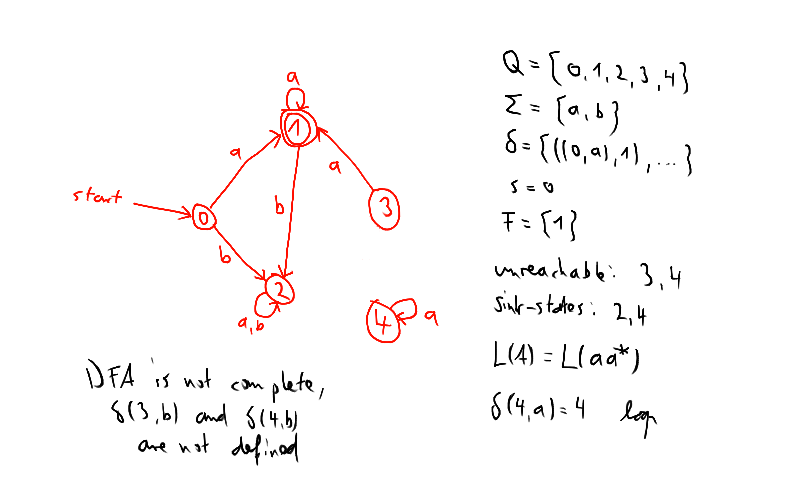
\includegraphics[width=\linewidth]{images/dfa.png}
	\caption{An example DFA and its properties.}
	\label{fig:dfa}
\end{figure}

\subsection{Minimal DFAs}

This section closely follows~\cite[pp. 42-45]{Sch01}. We call a DFA $A$ \emph{minimal}, if there exists no other automaton with the same language using less states. With $\mathfrak{A}_{min}$ we shall denote the set of all minimal DFAs.

The \emph{Nerode-relation} $\equiv_L\ \subseteq\ \Sigma^* \times \Sigma^*$ of a language $L$ with alphabet $\Sigma$ is defined as follows:
\begin{displaymath}
	x \equiv_L y\ \Leftrightarrow_{def}\ \forall z\in\Sigma^*\colon (xz\in L \Leftrightarrow yz\in L)
\end{displaymath}
The Nerode-relation of a DFA $A$ is the the Nerode-relation of its language: $\equiv_{L(A)}$. If the context makes it clear, than we will shorten the notation of a equivalence class $[x]_{\equiv_L}$ with $[x]$.

The \emph{equivalence class automaton} $A_L = (Q_L, \Sigma_L, \delta_L, s_L, F_L)$ to a regular language $L$ with alphabet $\Sigma$ is defined as follows:
\begin{itemize}
	\item $Q_L = \{\ [x]\ |\ x \in \Sigma^*\ \}$
	\item $\Sigma_L = \Sigma$
	\item $\delta_L([x], \sigma) = [x\sigma],\ \forall x\in\Sigma^*,\ \forall\sigma\in\Sigma$
	\item $s = [\varepsilon]$
	\item $F = \{\ [x]\ |\ x \in L\ \}$
\end{itemize}
\begin{theorem}
	Given a language $L$, then the equivalence class automaton $A_L$ is minimal.
\end{theorem}

\subsection{Practical Isomorphy of DFAs}

Given two DFAs $A_1 = (Q_1, \Sigma_1, \delta_1, s_1, F_1)$ and $A_2 = (Q_2, \Sigma_2, \delta_2, s_2, F_2)$. We say $A_1$ and $A_2$ are \emph{practical isomorph}, iff:
\begin{itemize}
	\item $|Q_1| = |Q_2|$, $|\Sigma_1| = |\Sigma_2|$ and
	\item there exists a bijection $\phi\colon \Sigma_1 \to \Sigma_2$ such that:
	\item there exists a bijection $\pi\colon Q_1 \to Q_2$ such that:
	
	$\pi(s_1) = s_2$
	
	$\forall q\in Q_1\colon (q\in F_1 \Longleftrightarrow \pi(q)\in F_2)$
	
	$\forall q\in Q_1\colon \forall\sigma\in\Sigma_1\colon \pi(\delta_1(q,\sigma))=\delta_2(\pi(q),\phi(\sigma)))$
\end{itemize}
Note that practical isomorphy between two DFAs $A_1, A_2$ does not imply $L(A_1) = L(A_2)$. This would be given, if $\Sigma_1 = \Sigma_2$ were the case (see~\cite[p. 45]{Sch01}). However the language of such DFAs is equivalent except for an exchange of alphabet symbols:
\[
	\{\ \phi(\sigma_0)\ldots\phi(\sigma_n)\ |\ \sigma_0\ldots\sigma_n\in L(A_1)\ \} = L(A_2)
\]
Practical isomorphy will be sufficient for our case. \gregor{why?}
%\begin{theorem} \textnormal{\cite[p. 45]{Sch01}} 
%	Every minimal DFA is unique except for isomorphy.
%\end{theorem}
%So it
%\begin{corollary}\label{ch:1:cor:all-min-dfa-ism}
%	Every minimal DFA $A$ is isomorph to its corresponding equivalence class automaton $A_{L(A)}$.
%	\gregor{All min. DFAs are ism. to each other, including A\_L}
%\end{corollary}
\gregor{Write down isomorphism test. Maybe discuss faster methods here? Look for faster methods in general?}

\subsection{Equivalent and distinguishable state pairs}

\begin{definition}[Equivalent and Distinguishable State Pairs]\cite[p. 154]{HMU01}
	A state pair $q_1, q_2 \in Q$ of a DFA $A = (Q, \Sigma, \delta, s, F)$ is called \emph{equivalent}, iff $\sim_A(q_1, q_2)$ is true, whereas
	\begin{displaymath}
	q_1\ \sim_A\ q_2 \Leftrightarrow_{def}\ \forall z \in \Sigma^* \colon\ (\delta^*(q_1, z) \in F \Leftrightarrow \delta^*(q_2, z) \in F)
	\end{displaymath}
	If $q_0 \not\sim_A q_1$, then $q_0$ and $q_1$ are called a \emph{distinguishable} state pair. The relation $\sim_A$ is an equivalence relation
\end{definition}
%\noindent Note the similarity between $\equiv_{L(A)}$ and $\sim_A$.:
%\begin{align*}
%	x\ \equiv_{L(A)}\ y\ \Leftrightarrow&\ \forall z\in\Sigma^*\colon (xz \in L \Leftrightarrow yz \in L) \\
%	& \\
%	q_1\ \sim_A\ q_2\ \Leftrightarrow&\ \forall z \in \Sigma^* \colon\ (\delta^*(q_1, z) \in F \Leftrightarrow \delta^*(q_2, z) \in F)
%\end{align*}
%We will prove the following statement regarding both relations:
%\begin{proposition}[Relationship of $\equiv_{L(A)}$ and $\sim_A$] \label{ch:1:prop-ner-eq} $ $ \\
%    \[
%    	x \equiv_{L(A)} y\ \Leftrightarrow\ \delta^*(s,x)=q_1\ \land\ \delta^*(s,y)=q_2\ \land\ q_1 \sim_A q_2
%    \]
%\end{proposition}
%\noindent Informally said: $x \equiv_{L(A)} y$ is true if and only if $q_1 \sim_A q_2$ whereas $q_1, q_2$ are reachable via $x,y$.
%\begin{proof} Via direct proof.
%    \begin{align*}
%    \ \delta^*(s,x)=q_1 \land \delta^*(s,y)=q_2\ \land\ & q_1 \sim_A q_2 \\
%    \Leftrightarrow\ \delta^*(s,x)=q_1 \land \delta^*(s,y)=q_2\ \land\ &(\forall z \in \Sigma^* \colon\ \delta^*(q_1, z) \in F \Leftrightarrow \delta^*(q_2, z) \in F) \\
%    \Leftrightarrow\hspace{5.65cm}&\ \forall z \in \Sigma^* \colon\ \delta^*(\delta^*(s,x), z) \in F \Leftrightarrow \delta^*(\delta^*(s,y), z) \in F \\
%    \Leftrightarrow\hspace{5.65cm}&\ \forall z \in \Sigma^* \colon\ \delta^*(s,xz) \in F \Leftrightarrow \delta^*(s,yz) \in F \\
%    \Leftrightarrow\hspace{5.65cm}&\ \forall z \in \Sigma^* \colon\ xz \in L(A) \Leftrightarrow yz \in L(A) \\
%    \Leftrightarrow\hspace{5.65cm}& x \equiv_{L(A)} y
%    \end{align*}
%\end{proof}
%\begin{corollary}
%    If the DFA $A$ is accessible, then there exists a $1:1$-correspondence between the equivalence classes of $\equiv_{L(A)}$ and $\sim_A$.
%\end{corollary}

%\noindent Proposition~\ref{ch:1:prop-ner-eq} can be supplemented by an even stronger declaration. Towards this declaration we first define, analogous to the equivalence class automaton, the \emph{$\sim$-equivalence automaton} $A_{\sim_A} = (Q_{\sim_A}, \Sigma_{\sim_A}, \delta_{\sim_A}, s_{\sim_A}, F_{\sim_A})$ to a DFA $A$:
%\begin{itemize}
%    \item $Q_{\sim_A} = \{[q]_{\sim_A} | q \in Q\}$
%    \item $\Sigma_{\sim_A} = \Sigma$
%    \item $\delta_{\sim_A}([q]_{\sim_A}, \sigma) = [\delta(q, \sigma)]_{\sim_A}, \forall q \in Q, \sigma \in \Sigma$
%    \item $s_{\sim_A} = [s]_{\sim_A}$
%    \item $F_{\sim_A} = \{[q]_{\sim_A} | q \in Q\}$
%\end{itemize}

%\begin{theorem}
%    If the DFA $A$ is accessible, then $A_{\sim_A}$ is minimal and thus isomorph to $A_L$.
%\end{theorem}

\subsection{The minimization algorithm}

This minimization algorithm \MinAlg\ works in four major steps, removing essentially states in such a way, that no unreachable states and no equivalent state pairs are left.
\begin{enumerate}
	\item Compute all unreachable states via breadth-first search.
	
	\vspace{0.2cm}
	\begin{algorithmic}[1]
		\Function{\CompUnr}{$A$}
			\State $U \gets Q \setminus \{s\}$	\Comment{undiscovered states}
			\State $O \gets \{s\}$				\Comment{observed states}
			\State $D \gets \{\}$				\Comment{discovered states}
			\While {$|O| > 0$}
				\State $N \gets \{\ p\ | \ \exists q \in O\ \sigma \in \Sigma \colon\ \delta(q, \sigma) = p\ \land\ p \notin O \cup D\ \}$
				\State $U \gets U \setminus N$
				\State $D \gets D \cup O$
				\State $O \gets N$
			\EndWhile
			\State \Return $U$
		\EndFunction
	\end{algorithmic}

	\item Remove all unreachable states and their transitions.
	
	\vspace{0.2cm}
	\begin{algorithmic}[1]
		\Function{\RemUnr}{$A, U$}
            \State $\delta' \gets \delta \setminus \{\ ((q,\sigma),p)\ |\ q\in U\ \lor\ p\in U\ \}$
			\State \Return $(Q \setminus U, \Sigma, \delta', s, F \setminus U)$
		\EndFunction
	\end{algorithmic}

	\item Compute all equivalent state pairs ($\sim_A$). Inspired by Schöning~\cite[p. 46]{Sch01} \gregor{And TI-VL}.
	
	\vspace{0.2cm}
	\begin{algorithmic}[1]
		\Function{\CompDist}{$A$} \label{ch:1:minmark}
		\State $M \gets \{ (p,q), (q,p)\ |\ p \in F, q \notin F \}$
		\Do
			\State $M' \gets \{ (p,q)\ |\ (p,q) \notin M \land \exists \sigma \in \Sigma \colon (\delta(p,\sigma), \delta(q,\sigma)) \in M \}$
			\State $M \gets M \cup M'$
		\doWhile {$M' \neq \emptyset$}
		\State \Return $Q^2 \setminus M$
		\EndFunction
	\end{algorithmic}
	Note that \CompDist\ requires its input automaton to be complete. \gregor{Why?}

	\item Merge all equivalent state pairs, which are exactly those in $\sim_A$. Inspired by Högberg~\cite[p. 10]{HL20}.
	
	\vspace{0.2cm}
	\begin{algorithmic}[1] \label{ch:1:minmerge}
		\Function{\RemEq}{$A$, $\sim_A$} \Comment{$[\cdot]_{\sim_A}$ shall be abbreviated $[\cdot]$}
            \State $Q_E \gets \emptyset$
            \State $\delta_E \gets \emptyset$
            \State $F_E \gets \emptyset$
            \For {$q$ \textbf{in} $Q$}
                \State Add $[q]$ to $Q_E$
                \For {$\sigma$ \textbf{in} $\Sigma$}
                    \State $\delta_E([q], \sigma) = [\delta(q, \sigma)]$
                \EndFor
                \If {$q \in F$}
                    \State Add $[q]$ to $F_E$
                \EndIf
            \EndFor
			\State \Return $(Q_E, \Sigma, \delta_E, [s], F_E)$
		\EndFunction
	\end{algorithmic}
	Note that \RemEq\ creates complete automatons.
\end{enumerate}

\vspace{0.2cm}
\begin{algorithmic}[1] \label{ch:1:minalg}
    \Function{\MinAlg}{$A_{task}$}
    \State $A_{re} \gets \RemUnr(A_{task}, \CompUnr(A_{task}))$
    \State $A_{sol} \gets \RemEq(A_{re}, \CompDist(A_{re}))$
    \State \Return $A_{sol}$
    \EndFunction
\end{algorithmic}
\vspace{0.2cm}
\noindent This DFA minimization algorithm has been found by Hopcroft~\cite{Hop71} and was established in teaching by Hopcroft et al.~\cite[pp. 154-164]{HMU01}.

\begin{theorem}\label{ch:1:min-alg-correct}\textnormal{\cite[pp. 162-164]{HMU01}}
	\MinAlg\ computes a minimal DFA to its input DFA.
\end{theorem}

\subsection{$m$-\CompDist.}

When looking at \CompDist, one notes, that it computes distinct subsets of $Q \times Q$ on the way. Indeed, one could write the algorithm in such a way, that these subsets are explicitly computed in form of a function $m\colon\mathbb{N}\to\mathcal{P}(Q\times Q)$:
\vspace{0.2cm}
\begin{algorithmic}[1] \label{ch:1:m-minmark}
	\Function{$m$-\CompDist}{$A$}
	\State $i \gets 0$
	\State $m(0) \gets \{ (p,q), (q,p)\ |\ p \in F, q \notin F \}$
	\Do
		\State $i \gets i + 1$
		\State $m(i) \gets \{ (p,q), (q,p)\ |\ (p,q) \notin \bigcup{m(\cdot)} \land \exists \sigma \in \Sigma \colon (\delta(p,\sigma), \delta(q,\sigma)) \in m(i-1) \}$
	\doWhile {$m(i) \neq \emptyset$}
	\State \Return $\bigcup{m(\cdot)}$
	\EndFunction
\end{algorithmic}
\vspace{0.2cm}
Using this redefinition, we can easier refer to the state pairs marked in a certain iteration. We will use both variants in exchange.

We will denote the number of iterations done by \CompDist\ on an DFA $A$ as $\mmD(A)$. Note that $\mmD(A) = \max n \in \mathbb{N}\ |\ m(n) \neq \emptyset$. \gregor{Does that note maybe fit very well to the proof of lemma~\ref{ch:3:semantics-of-D(A)}?}

%\subsection{\MinAlg-partition of a DFA}
%
%When looking at \MinAlg, one may note, that we can partition the states $Q_A$ of any DFA $A$ into three parts:
%\begin{itemize}
%	\item a subset of \emph{unreachable} states $U_A = \{\ u_1, \ldots, u_{\mathcal{Q}_{unr}}\ \}$ of size $\mathcal{Q}_{unr}$, found and removed in step 1 and 2
%	\item a subset of \emph{redundant} states $R_A = \{\ r_1, \ldots, r_{\mathcal{Q}_{eq}}\ \}$ of size $\mathcal{Q}_{eq}$, found and removed in step 3 and 4
%	\item a subset of \emph{essential} states $E_A = \{\ e_1, \ldots, e_\mathcal{Q}_{sol}\ \}$ of size $\mathcal{Q}_{sol}$, which are left over after applying the algorithm
%\end{itemize}
%Note that the set of essential states to a DFA is dependent on the implementation of \RemEq, but we know, that there will always be states left over, and for a given DFA the number will always be the same \gregor{why}.

%\gregor{Example: In~\ref{fig:dfa_ex_task} and~\ref{fig:dfa_ex_sol} the state pairs $(A,D), (C,E)$ are equivalent and all others distinguishable. The states $A, G, C, B$ are essential, for they show up in the minimized automaton. The states $D, E$ are therefore redundant.}

\subsection{Another equivalence automaton}

Consider step 3 and 4 of \MinAlg. A view on these algorithms reveal, that they are essentially collapsing each $\sim$-equivalence class of a DFA $A$ into one state.

\begin{definition}[$\sim_A$-equivalence automaton] \label{ch:1:sim-eq-dfa}
    We will call the automaton $E_A = (Q_E, \Sigma_E, \delta_E, s_E, F_E)$ created by \CompDist\ and \RemEq($A$)\ the \emph{$\sim_A$-equivalence automaton} of $A$. It has the following properties:
    \begin{itemize}
        \item $Q_E = \{\ [q]\ |\ q \in Q\ \}$
        \item $\Sigma_E = \Sigma$
        \item $\delta_E([q], \sigma) = [\delta(q, \sigma)], \forall q \in Q, \sigma \in \Sigma$
        \item $s_E = [s]_\sim$
        \item $F_E = \{\ [q]\ |\ q \in Q\ \}$
    \end{itemize}
    Note, that we know by theorem~\ref{ch:1:min-alg-correct} that $E_A$ is guaranteed to be a minimal automaton to $A$, if $A$ has no unreachable states.
\end{definition}

%Note moreover that, since $A_{sol}$ is minimal, there exists an isomorphism renaming $e_1,\ldots,e_\mathcal{Q}_{sol}$ such that they correspond to the equivalence classes of $\equiv_{L(A_{task})}\ = \ \equiv_{L(A_{re})}$ and $\sim_{A_{re}}$.
%
%However there might exist no isomorphism connecting $e_1,\ldots,e_\mathcal{Q}_{sol}$ and the equivalence classes of $\sim_{A_{task}}$, since possible unreachable states might form $\sim$-equivalence classes that are distinct to those of the reachable states.

\section{Requirements analysis}

Now that we have introduced all necessary basic definitions, we shall do a short analysis of an example DFA minimization task and its sample solution, as it could have been given to students in an introductory course to automata theory.

\subsection{Example of a DFA minimization task for students}

\gregor{search for typical task in standard text books}

\begin{figure}
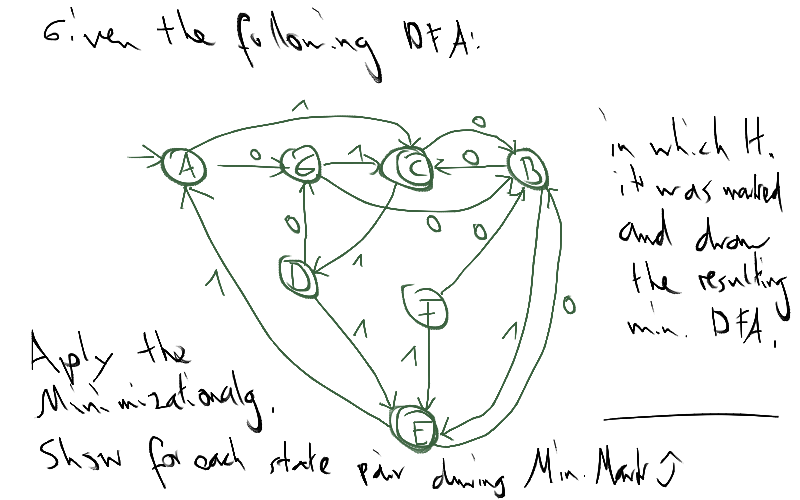
\includegraphics[width=\linewidth]{images/dfa_ex_task.png}
\caption{An example DFA minimization task.}
\label{fig:dfa_ex_task}
\end{figure}

\begin{figure}
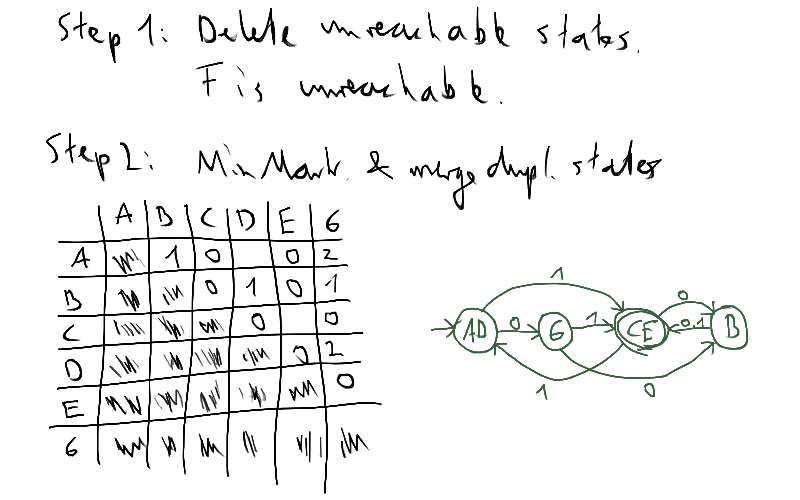
\includegraphics[width=\linewidth]{images/dfa_ex_sol.png}
\caption{Solution to the DFA minimization task in fig.~\ref{fig:dfa_ex_task}.}
\label{fig:dfa_ex_sol}
\end{figure}

\noindent Figures~\ref{fig:dfa_ex_task} and~\ref{fig:dfa_ex_sol} show such a task and solution. The students are confronted with a \emph{task DFA} $A_{task}$. Firstly, unreachable states have to be eliminated, we then gain the \emph{reachable DFA} $A_{re}$. Secondly equivalent state pairs of $A_{re}$ are merged such that the minimal \emph{solution DFA} $A_{sol}$ is found. The table $T$ displayed in figure~\ref{fig:dfa_ex_sol} is nothing else but a visualization of the function $m$, whereas $T(q_0, q_1) = i \Leftrightarrow (q_0, q_1) \in m(i)$.

We do some rather formal statements and requirements. Firstly, we can state that
\begin{itemize}
	\item $A_{re} = \RemUnr(A_{task}, \CompUnr(A_{task}))$ and
	\item $A_{sol} = \RemEq(A_{re}, \CompDist(A_{re}))$
\end{itemize}
Therefore $A_{sol}$ is minimal regarding $A_{re}$ and $A_{task}$. Secondly the languages of $A_{task}, A_{re}$ and $A_{sol}$ are be equal. We know that \CompDist\ requires $A_{re}$ to be complete and that \RemEq\ creates complete DFAs, so $A_{sol}$ is complete too. Furthermore we know that every state of $A_{re}$ is reachable since it is the output of \RemUnr.

\gregor{How to define 'already found DFA sol' as requirement. Final states argument missing.}

\subsection{Difficulty adjustment possibilities}

Concerning the execution of \MinAlg\ we find that its difficulty can be classified through various classification numbers.

\paragraph*{\CompDist-depth ($\mmD(A_{task})$).}

Consider the computation of the sets $m(i)$ in \CompDist. Determining $m(0)$ is quite straightforward, because it consists simply of tests whether two states are in $F \times Q \setminus F$ (see~\ref{ch:1:m-minmark}, line 3). Determining $m(1)$ is less easy: The rule for determining all $m(i), i > 0$ is different to that for $m(0)$ and more complicated (see~\ref{ch:1:m-minmark}, line 6). Determining $m(2)$ requires the same rule. It shows nonetheless a students understanding of the terminating behavior of \CompDist: It does not stop after computing $m(1)$, but only when no more distinguishable state pairs were found. Concerning the sets $m(i), i > 2$ however no additional understanding can be shown.

It would therefore be sensible if $\mmD(A_{task})$ could be adjusted for example by parameters $m_{min}, m_{max}$ which give lower and upper bounds for that value.

\paragraph*{Number of states ($\mathcal{Q}_{sol}, \mathcal{Q}_{eq}, \mathcal{Q}_{unr}$).}

To control the number of states in $A_{task}, A_{re}$ and $A_{sol}$, we will introduce three parameters: $\mathcal{Q}_{sol}, \mathcal{Q}_{eq}, \mathcal{Q}_{unr} \in \mathbb{N}$. These parameters get their meaning by the following equations:
\begin{align*}
    |Q_{sol}| &= \mathcal{Q}_{sol} \\
    |Q_{re}| &= \mathcal{Q}_{sol} + \mathcal{Q}_{eq} \\
    |Q_{task}| &= \mathcal{Q}_{sol} + \mathcal{Q}_{eq} + \mathcal{Q}_{unr}
\end{align*}
It is sensible to have $\mathcal{Q}_{unr} > 1, \mathcal{Q}_{eq} > 1$, such that \RemUnr\ and \RemEq\ will not be skipped. To not make the task trivial, $\mathcal{Q}_{sol} > 2$ is sensible. An exercise instructor will find it useful, to control exactly how big $\mathcal{Q}_{unr}$, $\mathcal{Q}_{eq}$ and $\mathcal{Q}_{sol}$ are: The higher $\mathcal{Q}_{unr}, \mathcal{Q}_{eq}$, the more states have to be eliminated and merged. The higher $\mathcal{Q}_{sol} + \mathcal{Q}_{eq}$, the more state pairs have to be checked during \CompDist.

\gregor{Concept for min max.}
%To control the number of states in $A_{task}, A_{re}$ and $A_{sol}$, we will introduce three pairs of parameters, denoting each ranges: $Q_{s,min}, Q_{s,max}$ for the number of states in the solution DFA, $Q_{e,min}, Q_{e,max}$ for the number of equivalent state pairs in $A_{re}$ and $A_{task}$, and $Q_{u,min}, Q_{u,max}$ for the number of unreachable states in $A_{task}$. Consequently the following equations are true:
%\begin{align*}
%|Q_{sol}| &\in [Q_{s,min}, Q_{s,max}] \\
%|Q_{re}| &= |Q_{sol}| + n \in [Q_{e,min}, Q_{e,max}] \\
%|Q_{task}| &= |Q_{re}| + n \in [ Q_{u,min}, Q_{u,max}]
%\end{align*}

\paragraph*{Alphabet size.}

The more symbols the alphabet of $A_{task}, A_{re}$ and $A_{sol}$ has (note how \MinAlg\ does not change the alphabet), the more transitions have to be followed when checking whether $(\delta(q,\sigma),\delta(p,\sigma))\in m(i-1)$ is true for each state pair $p,q$.

\paragraph*{Completeness of $A_{task}$.}

Even though \CompUnr\ and \RemUnr\ do not require their input DFA $A_{task}$ to be complete, it is sensible to build it that way. The implications of the completeness-property are - in comparison to the other concepts involved here - rather subtle. This is especially due to its purely representational nature, a DFA has the same language and $\mmD$-value, whether it is represented in its complete form or not. Nonetheless we shall introduce a parameter $c$, that determines if there exist unreachable states, that make $A_{task}$ incomplete. Thus an exercise lecturer could showcase this matter on a DFA and generate according exercises.

\paragraph*{Planar drawing of $A_{task}$.}

A graph $G$ is \emph{planar} if it can be represented by a drawing in the plane such that its edges do not cross. Such a drawing is then called \emph{planar drawing} of $G$. A visual aid for students would be given, if the task DFA were planar and presented as a planar drawing. In this work libraries and parameters $p_1, p_2 \in \{0,1\}$ (toggling planarity of $A_{sol}, A_{task}$) will be used to allow the option of planarity, but neither ensuring planarity nor planar drawing will be investigated further theoretically.

\paragraph*{Maximum degree of any state in $A_{task}$.}

The \emph{degree} $deg(q)$ of a state $q \in Q$ in a DFA $A$ is defined as $deg(q) = |d^-(q)| + |d^+(q)|$, so the total number of transitions in which $q$ participates. By capping the maximum degree for all states, the graphical representation of the DFA would be more clear. In this work the inclusion of a maximum degree parameter is omitted.

%Note that $deg(q) \geq |\Sigma|$ for any complete DFA, since states of complete DFAs have to use all alphabet symbols on outgoing transitions.

\subsection{Summary of found criteria}

\gregor{TODO}

\label{ch:1:determined-requirements}
Accepted general criteria:
\begin{itemize}
	\item[->] $L(A_{sol}) = L(A_{re}) = L(A_{task})$
	\item[->] $\mmD(A_{sol}) = \mmD(A_{re}) = \mmD(A_{task})$
\end{itemize}
Accepted solution DFA criteria:
\begin{itemize}
	\item[->] has to be minimal, complete
	\item[->] number of essential states
	\item[->] number of \CompDist\ iterations ($\mmD(A_{sol})$)
	\item[->] alphabet size
	\item[->] number of accepting states
	\item[->] planarity
	\item[->] $A_{sol}$ is new
	
	\begin{definition}[New DFAs] \label{ch:1:new-dfa}
		A DFA $A_{sol}$ is \emph{new} if it is not practically isomorph to any previously generated solution DFA.
	\end{definition}
\end{itemize}
Accepted reachable DFA criteria:
\begin{itemize}
	\item[->] has to be complete
	\item[->] number of unreachable states
	\item[->] planarity (can be checked in $O(|Q_{task}|)$)
\end{itemize}
Accepted task DFA criteria:
\begin{itemize}
	\item[->] number of states that are added to create equivalent state pairs
	\item[->] planarity
	\item[->] completeness
\end{itemize}

\section{Approach and general algorithm}

In this work we will first build the solution DFA (step 1), and - based on that - the task DFA by creating equivalent states and adding unreachable states (step 2). Both steps will fulfill all criteria chosen above and are covered in depth in chapter~\ref{ch:2} respectively chapter~\ref{ch:3}.

It follows that $\mmD$ and $L$ of both DFAs will be set when building $A_{sol}$. We know that creating equivalent states and adding unreachable does not change $L(A_{task})$ in comparison to $A_{sol}$, else \MinAlg\ would not work (a minimal DFA has in particular the same language as the original DFA). However we must ensure, that adding those states does not change $\mmD$. Since unreachable states are eliminated before \CompDist\ is applied, we need only to ensure, that creating equivalent states does not change the $\mmD$-value. We will do this during the discussion of step 2, more specifically in section~\ref{ch:3:sec-D-proof}.

At the beginning of chapter 2 and 3, we will provide formal problem definitions for both steps, that specify precisely all requirements. Here we shall content ourselves with the definition of the main algorithm:
\vspace{0.2cm}
\begin{algorithmic}[1]
	\Function{GenerateDFAMinimizationProblem}{$\mathcal{Q}_{sol}, a, f, m_{min}, m_{max}, p_1, p_2, \mathcal{Q}_{eq},\mathcal{Q}_{unr}, c$}
	\State $A_{sol} \gets \textsc{GenerateNewMinimalDFA}(\mathcal{Q}_{sol}, a, f, m_{min}, m_{max}, p_1)$
	\State $A_{task} \gets \textsc{ExtendMinimalDFA}(A_{sol}, p_2, \mathcal{Q}_{eq},\mathcal{Q}_{unr}, c)$
	\State \Return $A_{sol}, A_{task}$
	\EndFunction
\end{algorithmic}



	% !TeX spellcheck = en_US

\chapter{Problem definition and approach} \label{ch:2}

In this chapter we will set foundations, investigate sensible parameters and requirements for a minimization task generator and deduce our general approach to build such a program.

\section{Preliminaries}

We start with defining preliminary theoretical foundations. By $[[n]]$ we will denote the set of integers $\{0,\ldots,n-1\}$.

\subsection{Deterministic Finite Automatons}

A 5-tuple $A = (Q, \Sigma, \delta, s, F)$ with $Q$ being a finite set of \emph{states}, $\Sigma$ a finite set of \emph{alphabet symbols}, $\delta \colon\ Q \times \Sigma \to Q$ a \emph{transition function}, $s \in Q$ a \emph{start state} and $F \subseteq Q$ \emph{final states} is called \emph{deterministic finite automaton} (DFA)~\cite[p. 46]{HMU01}. From now on $\A$ shall denote the set of all DFAs.

We say $\delta(q,\sigma) = p$ is a transition from $q$ to $p$ using symbol $\sigma$. We define the \emph{extended transition function} $\delta^* : Q \times \Sigma^* \to Q$ of a DFA $A = (Q, \Sigma, \delta, s, F)$ as:
\begin{itemize}
	\item $\delta^*(q,\varepsilon) = q$
	\item $\delta^*(q,w\sigma) = \delta(\delta^*(q,w),\sigma)$ for all $q \in Q$, $w \in \Sigma^*$, $\sigma \in \Sigma$
\end{itemize}
Then, the \emph{language} of $A$ is defined as $L(A) = \{\ w\ |\ \delta^*(w) \in F\ \}$~\cite[pp. 49-50. 52]{HMU01}.

Given a state $q \in Q$. With $d^-(q)$ we denote the set of all \emph{ingoing} transitions $\delta(q', \sigma) = q$ of $q$. With $d^+(q)$ we denote the set of all \emph{outgoing} transitions $\delta(q, \sigma) = q'$ of $q$~\cite[pp. 2-3]{CP05}.

\begin{definition}[(Un-)Reachable State]\label{ch:2:unreachable-states}
	We say a state $q$ is \emph{(un-)reachable} in a DFA $A$, iff there is (no) a word $w \in \Sigma^*$ such that $\delta^*(s, w) = q$.
\end{definition}
\noindent If all states of a DFA $A$ are reachable, then we call $A$ \emph{accessible}~\cite[p. 2]{CP05}.

A DFA is called \emph{complete} iff for all states, every symbol of the alphabet is used on an outgoing transition: $\forall q\in Q\colon \forall\sigma\in\Sigma\colon \exists p\in Q\colon \delta(q,\sigma) = p$. Note, that every incomplete DFA can be converted to a complete one by adding a so called \emph{dead state}~\cite[p. 67]{HMU01}. The resulting automaton has the same language. From now on we will only work with complete DFAs.

\begin{figure}[H]
	\begin{subfigure}{.5\textwidth}\centering\resizebox{1.\linewidth}{!}{
		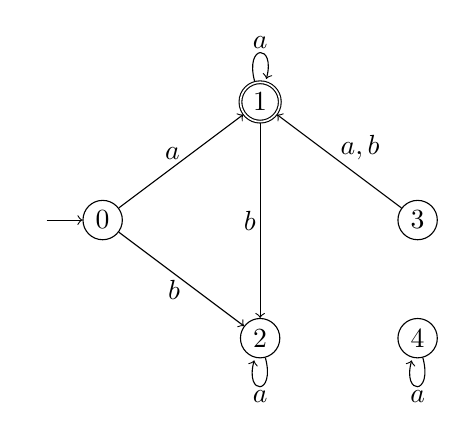
\begin{tikzpicture}[initial text={},scale=1., every node/.style={transform shape}]
		\tikzstyle{every state}=[minimum size=5mm, inner sep=0pt]
		
		\node[initial, state]  (0) at (0, 0) {$0$};
		\node[accepting,state] (1) at (2, 1.5) {$1$};
		\node[state]           (2) at (2,-1.5) {$2$};
		\node[state]           (3) at (4, 0) {$3$};
		\node[state]           (4) at (4,-1.5) {$4$};
		
		\path[->]
		(0) edge 			  node [above left=-0.15cm]  {$a$}   (1)
		(1) edge [loop above] node [above=-0.07cm]		 {$a$}   (1)
		(1) edge 			  node [left=-0.07cm]        {$b$}   (2)
		(0) edge 			  node [below left=-0.15cm]  {$b$}   (2)
		(2) edge [loop below] node [below=-0.07cm]       {$a$}   (2)
		(3) edge 			  node [above right=-0.15cm] {$a,b$} (1)
		(4) edge [loop below] node [below=-0.07cm]	     {$a$}   (4)
		;
		\end{tikzpicture}
	}\end{subfigure}
	\hfill
	\begin{subfigure}{.4\textwidth}
		\begin{align*}
			&A = (Q, \Sigma, \delta, s ,F) \\
			&\\
			&Q = [[5]] = \{\ 0,1,2,3,4\ \} \\
			&\Sigma = \{\ a,b\ \} \\
			&\delta = \{\ ((0,a),1), ((0,b),2), \ldots\ \} \\
			&s = 0 \\
			&F = \{\ 1\ \}
		\end{align*}
	\end{subfigure}
	\caption{An example DFA. The states $3$ and $4$ are unreachable. This DFA is not complete since the transitions $\delta(2,b)$ and $\delta(4,b)$ are not defined.}
	\label{fig:dfa}
\end{figure}

\begin{definition}[Minimal DFA]
	We call a DFA $A$ \emph{minimal}, if there exists no other DFA with the same language having less states.
\end{definition}
\noindent With $\Amin$ we shall denote the set of all minimal DFAs.

\begin{definition}[Equivalent and Distinguishable State Pairs]\cite[p. 154]{HMU01}\label{ch:2:def:eq-dist-pairs}
	A state pair $q_1, q_2 \in Q$ of a DFA $A = (Q, \Sigma, \delta, s, F)$ is called \emph{equivalent}, iff $\sim_A(q_1, q_2)$ is true, where
	\begin{displaymath}
	q_1 \sim_A q_2 \text{ is true}\ \Leftrightarrow_{def}\ \forall z \in \Sigma^* \colon\ (\delta^*(q_1, z) \in F \Leftrightarrow \delta^*(q_2, z) \in F)
	\end{displaymath}
	If $q_0 \not\sim_A q_1$, then $q_0$ and $q_1$ are called a \emph{distinguishable} state pair. It is well-known (see for instance~\cite[p. 160]{HMU01}) that the relation $\sim_A$ is an equivalence relation.
\end{definition}

\subsection{Isomorphy of DFAs}\label{ch:2:sec:isom}

Given two DFAs $A_1 = (Q_1, \Sigma_1, \delta_1, s_1, F_1)$ and $A_2 = (Q_2, \Sigma_2, \delta_2, s_2, F_2)$. We say $A_1$ and $A_2$ are \emph{isomorphic}, iff:
\begin{itemize}
	\item $|Q_1| = |Q_2|$, $\Sigma_1 = \Sigma_2$ and
	\item there exists a bijection $\pi\colon Q_1 \to Q_2$ such that:
	
	$\pi(s_1) = s_2$
	
	$\forall q\in Q_1\colon (q\in F_1 \Longleftrightarrow \pi(q)\in F_2)$
	
	$\forall q\in Q_1\colon \forall\sigma\in\Sigma_1\colon \pi(\delta_1(q,\sigma))=\delta_2(\pi(q),\sigma))$
\end{itemize}
In~\cite[p. 45]{Sch01} we can find the following statement:
\begin{theorem}\label{ch:2:thm:uniq-ism}
	Every minimal DFA is unique (has a unique language) except for isomorphy.
\end{theorem}
\noindent We describe a simple isomorphism test for DFAs in appendix~\ref{ch:app:ism-test}.

\subsection{Hopcroft's Minimization Algorithm}

There are three major algorithms for DFA minimization found by Moore, Brzozowski and Hopcroft, respectively (\cite[p. 2]{BBC10}). On the latter an easy algorithm is based, that is presented in the textbook~\cite{HMU01} and will be described here more precisely. We will call Hopcroft's algorithm `the minimization algorithm' from now on. Its general structure is the following:
\vspace{0.2cm}
\begin{algorithmic}[1] \label{ch:2:minalg}
	\Function{\MinAlg}{$A$}
	\State $A' \gets \RemUnr(A, \CompUnr(A))$
	\State \Return $\RemEq(A', \CompDist(A'))$
	\EndFunction
\end{algorithmic}
\vspace{0.2cm}

\noindent It can be seen that \MinAlg\ works in four major steps. In step 1 and 2 unreachable states are found and removed. In step 3 all equivalent state pairs are found. Step 4 removes states in such a way, that no equivalent state pairs are left.
\begin{enumerate}
	\item Compute all unreachable states via breadth-first search.
	
	\vspace{0.2cm}
	\begin{algorithmic}[1]
		\Function{\CompUnr}{$A$}
			\State $U \gets Q \setminus \{s\}$	\Comment{undiscovered states}
			\State $O \gets \{s\}$				\Comment{observed states}
			\State $D \gets \{\}$				\Comment{discovered states}
			\While {$|O| > 0$}
				\State $N \gets \{\ p\ | \ \exists q \in O\ \sigma \in \Sigma \colon\ \delta(q, \sigma) = p\ \land\ p \notin O \cup D\ \}$
				\State $U \gets U \setminus N$
				\State $D \gets D \cup O$
				\State $O \gets N$
			\EndWhile
			\State \Return $U$
		\EndFunction
	\end{algorithmic}

	\item Remove all unreachable states and their transitions.
	
	\vspace{0.2cm}
	\begin{algorithmic}[1]
		\Function{\RemUnr}{$A, U$}
            \State $\delta' \gets \delta \setminus \{\ ((q,\sigma),p)\in\delta\ |\ q\in U\ \lor\ p\in U\ \}$
			\State \Return $(Q \setminus U, \Sigma, \delta', s, F \setminus U)$
		\EndFunction
	\end{algorithmic}

	\item Compute all equivalent state pairs ($\sim_A$). The representation is inspired by Martens and Schwentick~\cite[ch.~4, p.~17]{MS18}. Note that \CompDist\ requires its input automaton to be complete (\cite[p.~13]{BBC10}).
	\vspace{0.2cm}
	\begin{algorithmic}[1]
		\Function{\CompDist}{$A$} \label{ch:2:minmark}
		\State $M \gets \{ (p,q), (q,p)\ |\ p \in F, q \notin F \}$
		\Do
			\State $M' \gets \{ (p,q)\ |\ (p,q) \notin M \land \exists \sigma \in \Sigma \colon (\delta(p,\sigma), \delta(q,\sigma)) \in M \}$
			\State $M \gets M \cup M'$
		\doWhile {$M' \neq \emptyset$}
		\State \Return $Q^2 \setminus M$
		\EndFunction
	\end{algorithmic}

	\item Merge all equivalent state pairs, which are exactly those in $\sim_A$. The representation is inspired by Högberg and Larsson~\cite[p.~10]{HL20}.
	
	\vspace{0.2cm}
	\begin{algorithmic}[1] \label{ch:2:minmerge}
		\Function{\RemEq}{$A$, $\sim_A$}
            \State $Q' \gets \emptyset, \delta' \gets \emptyset, F' \gets \emptyset$
            \For {$q$ \textbf{in} $Q$}
                \State Add $[q]$ to $Q'$ \Comment{$[\cdot]_{\sim_A}$ shall be abbreviated $[\cdot]$}
                \For {$\sigma$ \textbf{in} $\Sigma$}
                    \State $\delta'([q], \sigma) = [\delta(q, \sigma)]$
                \EndFor
                \If {$q \in F$}
                    \State Add $[q]$ to $F'$
                \EndIf
            \EndFor
			\State \Return $(Q', \Sigma, \delta', [s], F')$
		\EndFunction
	\end{algorithmic}
\end{enumerate}
The following theorem states the most important property of \MinAlg.

\begin{theorem}\label{ch:2:min-alg-correct}\textnormal{\cite[pp. 162-164]{HMU01}}
	\MinAlg\ computes a minimal DFA to its input DFA.
\end{theorem}

\noindent When looking at \CompDist, one notes, that it computes distinct subsets of $Q \times Q$ on the way. Indeed, one could write the algorithm in such a way, that these subsets are explicitly computed in form of a function $m\colon\mathbb{N}\to\mathcal{P}(Q\times Q)$:
\vspace{0.2cm}
\begin{algorithmic}[1] \label{ch:2:m-minmark}
	\Function{\mCompDist}{$A$}
	\State $i \gets 0$
	\State $m(0) \gets \{ (p,q), (q,p)\ |\ p \in F, q \notin F \}$
	\Do
		\State $i \gets i + 1$
		\State $m(i) \gets \{ (p,q), (q,p)\ |\ (p,q) \notin \bigcup{m(\cdot)} \land \exists \sigma \in \Sigma \colon (\delta(p,\sigma), \delta(q,\sigma)) \in m(i-1) \}$
	\doWhile {$m(i) \neq \emptyset$}
	\State \Return $\bigcup{m(\cdot)}$
	\EndFunction
\end{algorithmic}
\vspace{0.2cm}
Using this redefinition, we can easier refer to the state pairs marked in a certain iteration. We will use both variants of \CompDist\ in exchange.
\begin{definition}\label{ch:2:def:D(A)}
	We denote the number of iterations done by \CompDist\ on a DFA $A$ as $\mmD(A)$.
\end{definition}
\noindent This number will prove to be a major characteristic of difficulty for a minimization task.

\section{DFA Minimization Problems}

Now that we have introduced all necessary basic definitions, we present an example DFA minimization task and its sample solution, as it could have been given to students in an introductory course on automata theory. In this context further naming conventions will be determined.

\begin{figure}[ht]
	{\raggedright\itshape \underline{Task:} Consider the below shown deterministic finite automaton $A$:}
	\begin{center}\resizebox{.75\linewidth}{!}{
		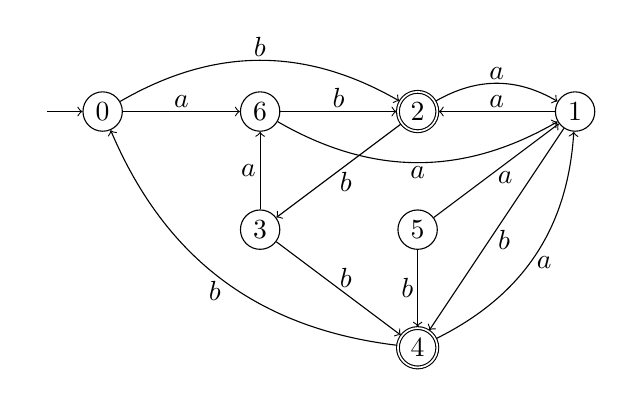
\begin{tikzpicture}[initial text={},scale=1., every node/.style={transform shape}]
		\tikzstyle{every state}=[minimum size=5mm, inner sep=0pt]
		
		\node[initial, state]  (0) at (0, 0)    {$0$};
		\node[state] 		   (1) at (6, 0)    {$1$};
		\node[state,accepting] (2) at (4,0)     {$2$};
		\node[state]           (3) at (2, -1.5) {$3$};
		\node[state,accepting] (4) at (4,-3)    {$4$};
		\node[state]           (5) at (4,-1.5)  {$5$};
		\node[state]           (6) at (2,0)     {$6$};
		
		\path[->]
		(0) edge node [above=-0.07cm]  {$a$}   (6)
		(0) edge [bend left] node [above=-0.07cm]  {$b$}   (2)
		
		(1) edge node [above=-0.07cm]  {$a$}   (2)
		(1) edge node [below right=-0.15cm]  {$b$}   (4)
		
		(2) edge [bend left] node [above=-0.07cm]  {$a$}   (1)
		(2) edge node [below right=-0.15cm]  {$b$}   (3)
		
		(3) edge node [left=-0.07cm]  {$a$}   (6)
		(3) edge node [above right=-0.15cm]  {$b$}   (4)
		
		(4) edge [bend right] node [below right=-0.15cm]  {$a$}   (1)
		(4) edge [bend left] node [below left=-0.15cm]  {$b$}   (0)
		
		(5) edge node [below right=-0.15cm]  {$a$}   (1)
		(5) edge node [left=-0.07cm]  {$b$}   (4)
		
		(6) edge [bend right] node [below=-0.07cm]  {$a$}   (1)
		(6) edge node [above=-0.07cm]  {$b$}   (2)
		;
		\end{tikzpicture}
	}\end{center}
	\itshape Apply the minimization algorithm and illustrate for each state pair of $A$ during which \CompDist-iteration it was marked. Draw the resulting automaton.
	\caption{An example DFA minimization task.}
	\label{fig:dfa_ex_task}
\end{figure}

\begin{figure}[ht]
	{\raggedright\itshape \underline{Solution:}\newline
		Step 1: Detect and eliminate unreachable states.
		\begin{tabbing}
			\qquad\textnormal{State $5$ is unreachable.}
		\end{tabbing}
		Step 2: Apply \CompDist\ to $A$ and merge equivalent state pairs:\par
	}
	\begin{subfigure}{.4\textwidth}
		\vspace{0.5cm}
		\qquad
		\begin{tabular}{c|c|c|c|c|c|c}
			  & 0  & 1  & 2  & 3  & 4  & 6  \\\hline
			0 & \x & 1  & 0  &    & 0  & 2  \\\hline
			1 & \x & \x & 0  & 1  & 0  & 1  \\\hline
			2 & \x & \x & \x & 0  &    & 0  \\\hline
			3 & \x & \x & \x & \x & 0  & 2  \\\hline
			4 & \x & \x & \x & \x & \x & 0  \\\hline
			6 & \x & \x & \x & \x & \x & \x \\
		\end{tabular}
	\end{subfigure}
	\begin{subfigure}{.5\textwidth}\centering\resizebox{1.\linewidth}{!}{
		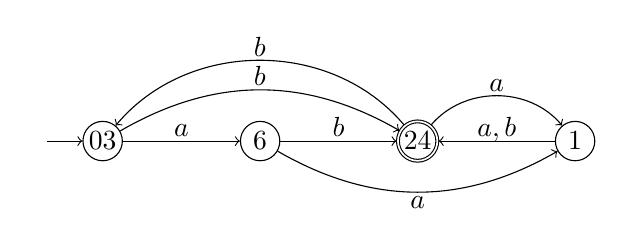
\begin{tikzpicture}[initial text={},scale=1., every node/.style={transform shape}]
		\tikzstyle{every state}=[minimum size=5mm, inner sep=0pt]
		
		\node[initial, state]  (03) at (0, 0)   {$03$};
		\node[state] 		   (1) at (6, 0)   {$1$};
		\node[state,accepting] (24) at (4,0)    {$24$};
		\node[state]           (6) at (2,0)    {$6$};
		
		\path[->]
		(03) edge node [above=-0.07cm]  {$a$}   (6)
		(03) edge [bend left] node [above=-0.07cm]  {$b$}   (24)
		
		(1) edge node [above=-0.13cm]  {$a,b$}   (24)
		
		(24) edge [bend left=50] node [above=-0.07cm]  {$a$}   (1)
		(24) edge [bend right=50] node [above=-0.07cm]  {$b$}   (03)
		
		(6) edge [bend right] node [below=-0.07cm]  {$a$}   (1)
		(6) edge node [above=-0.07cm]  {$b$}   (24)
		;
		\end{tikzpicture}
	}\end{subfigure}
	\caption{Solution to the DFA minimization task in fig.~\ref{fig:dfa_ex_task}.}
	\label{fig:dfa_ex_sol}
\end{figure}

\noindent Figures~\ref{fig:dfa_ex_task} and~\ref{fig:dfa_ex_sol} show a DFA minimization task and its solution. The students are confronted with a \emph{task DFA} $A_{task}$, which has to be minimized --- we will assume that Hopcroft's algorithm is used.

As a consequence (following alg.~\ref{ch:2:minalg}) firstly, unreachable states have to be eliminated, we then gain $A_{re}$ (having only \emph{reachable} states). Secondly equivalent state pairs of $A_{re}$ are merged such that the minimal \emph{solution DFA} $A_{sol}$ is found. The table $T$ displayed in Figure~\ref{fig:dfa_ex_sol} is nothing else but a visualization of the function $m$ of \mCompDist, where $T(q_0, q_1) = i \Leftrightarrow (q_0, q_1) \in m(i)$.

Notice that step 2 and in particular the computation of $\sim_A$ can be seen as central: Step 1 is relatively easy, unreachable states can normally be detected visually without running a search algorithm. Moreover algorithms like breadth-first search are often introduced earlier in computer science education. In step 2 computing $\sim_A$ is conceptually harder to grasp than collapsing $A_{re}$ towards the solution DFA.

We will call a pair $A_{sol}, A_{task}$ with $A_{sol} = \MinAlg(A_{task})$ a \emph{DFA minimization problem}. Our goal in this thesis is to automatically generate such problems. Before starting to think about concrete generation algorithms, we will devise some parameters and requirements.

\section{Requirements and Parameters for a Generation Algorithm}\label{ch:2:requirements-analysis}

Of some simple requirements we already know in advance. Firstly, we can state that $A_{sol}$ has to be minimal regarding $A_{re}$ and $A_{task}$. Secondly the languages of $A_{task}, A_{re}$ and $A_{sol}$ must be the same. Lastly we know that every state of $A_{re}$ needs to be reachable.

% Difficulty adjustment possibilities

Besides some other sensible requirements we will devise especially parameters for generation algorithms in this section. These parameters are going to be adjustment possibilities, which will in almost all cases allow to influence the difficulty of the generated problem in some way.

Since the difficulty of a DFA minimization task $A_{task}$ for students is mainly determined by the difficulty of executing \MinAlg$(A_{task})$, most parameters will influence certain aspects of the execution of \MinAlg.

\paragraph*{\CompDist-iterations ($d$).}

Consider the computation of the sets $m(i)$ in \mCompDist\ (see alg.~\ref{ch:2:m-minmark}). Determining $m(0)$ is quite straightforward, because it consists simply of tests whether two states are in $F \times Q \setminus F$ (see line 3). Determining $m(1)$ is less easy: The rule for determining all $m(i), i > 0$ is different to that for $m(0)$ and more complicated (see line 6). Determining $m(2), m(3), \ldots$ requires the same rule. It shows nonetheless a students understanding of \CompDist' terminating behavior: The algorithm does not stop after computing $m(1)$, but only when no more distinguishable state pairs were found.

It would therefore be sensible if $\mmD(A_{task})$ could be adjusted by some parameter $d$.

\paragraph*{Number of states \texorpdfstring{($\nSO, \nEQ, \nUN$)}{}.}

To control the number of states in $A_{task}, A_{re}$ and $A_{sol}$, we will introduce three parameters: $\nSO, \nEQ, \nUN \in \mathbb{N}$, where
\begin{itemize}
	\item $\nSO$ is the number of states of the \emph{solution} DFA $A_{sol}$
	\item $\nEQ$ is the number of distinct \emph{equivalent} state pairs of $A_{re}$
	\item $\nUN$ is the number of \emph{unreachable} states of $A_{task}$
\end{itemize}
They can be equivalently described by the following equations:
\begin{align*}
    |Q_{sol}| &= \nSO \\
    |Q_{re}| &= \nSO + \nEQ \\
    |Q_{task}| &= \nSO + \nEQ + \nUN
\end{align*}
It is sensible to have $\nUN > 1, \nEQ > 1$, such that \RemUnr\ and \RemEq\ will not be skipped. To not make the task trivial, $\nSO > 2$ is sensible. An exercise instructor will find it useful to control exactly how big $\nUN$, $\nEQ$ and $\nSO$ are: The higher $\nUN, \nEQ$, the more states have to be eliminated and merged. The higher $\nSO + \nEQ$, the more state pairs have to be checked during \CompDist.

\paragraph*{Alphabet size \texorpdfstring{($\kAL$)}{}.}

The more symbols the alphabet of $A_{task}, A_{re}$ and $A_{sol}$ has (note that \MinAlg\ does not change the alphabet), the more transitions have to be followed when checking whether $(\delta(q,\sigma),\delta(p,\sigma))\in m(i-1)$ is true for each state pair $p,q$ (see line 6 of alg.~\ref{ch:2:m-minmark}). In addition we will see later, that there exists no DFA with $k<2$ having any equivalent state pairs, so $k\ge 2$ is sensible and even required if $\nEQ > 0$.

\paragraph*{Number of final states \texorpdfstring{($\nF$)}{}.}

Most DFAs in teaching have about 1 to 3 final states (see e.g.~\cite[pp. 48-78]{HMU01} or~\cite[pp. 28-48]{Sch01}), so being able to set a number of final states allows concentrating on or deviating from familiar DFAs.

In this work $\nF$ shall determine the number of final states in $A_{sol}$. As a consequence, $A_{task}$ might have minimum $\nF$ and maximum $\nF + \nEQ + \nUN$ final states. The latter is the case, if all equivalent states are created from final states and if every unreachable state is created as final state.

\paragraph*{Uniqueness of solution DFA language.}

For example for an exam it would be sensible to be able to generate a task where the DFA language is unique, meaning there was no previously generated DFA with the same language.

Note that, if $A_{sol}$ is indeed \emph{new} in that sense, then $A_{task}$ will automatically have a unique language too, since $A_{sol}$ and $A_{task}$ always have the same language.

\paragraph*{Completeness of task DFA \texorpdfstring{($c$)}{}.}

In opposition to \CompDist, \CompUnr\ and \RemUnr\ do not require their input DFA $A_{task}$ to be complete. So we could have unreachable states in $A_{task}$, to which $\delta$ is not defined for all alphabet symbols. It is however sensible, to build task DFAs complete too to avoid possible confusion: Such subtleties do not highlight the main ideas of \MinAlg.

Nonetheless we shall introduce a boolean parameter $c$, that determines if there exist unreachable states, that make $A_{task}$ incomplete. Thus an exercise lecturer has the option, to showcase this matter on a DFA and generate according exercises.

\paragraph*{Planar drawing of task DFA \texorpdfstring{($p_{sol}, p_{task}$)}{}.}

A graph $G$ is \emph{planar} if it can be represented by a drawing in the plane such that its edges do not cross. Such a drawing is then called \emph{planar drawing} of $G$. A visual aid for students would be given, if the task DFA were planar and presented as a planar drawing. In this work libraries and parameters $p_{sol}, p_{task} \in \{0,1\}$ (toggling planarity of $A_{sol}, A_{task}$) will be used to allow the option of planarity, but neither ensuring planarity nor planar drawing will be investigated further theoretically.

\paragraph*{Maximum degree of any state in task DFA.}

The \emph{degree} $deg(q)$ of a state $q \in Q$ in a DFA $A$ is defined as $deg(q) = d^-(q) + d^+(q)$, so the total number of transitions in which $q$ participates. By capping the maximum degree for all states, the graphical representation of the DFA would be more clear. Here the inclusion of a maximum degree parameter is omitted.

%Note that $deg(q) \geq |\Sigma|$ for any complete DFA, since states of complete DFAs have to use all alphabet symbols on outgoing transitions.

\section{Approach and General Algorithm}

We will first build the solution DFA (step 1), and - based on that - the task DFA by creating equivalent states and adding unreachable states (step 2). Both steps together will fulfill all criteria chosen above and are covered each in depth in chapter~\ref{ch:3} respectively chapter~\ref{ch:4}.

At the beginning of chapter~\ref{ch:3} and~\ref{ch:4}, we will provide formal problem definitions for both steps, that specify precisely all requirements. Here we shall content ourselves with the definition of the main algorithm:
\vspace{0.2cm}
\begin{algorithmic}[1]
	\Function{GenDFAMinProblem}{$\nSO, \kAL, \nF, d, p_{sol}, p_{task}, \nEQ,\nUN, c$}
	\State $A_{sol} \gets \textsc{GenNewMinDFA}(\nSO, \kAL, \nF, d, p_{sol})$
	\State $A_{task} \gets \textsc{ExtendMinDFA}(A_{sol}, p_{task}, \nEQ, \nUN, c)$
	\State \Return $A_{sol}, A_{task}$
	\EndFunction
\end{algorithmic}
\vspace{0.2cm}
\noindent One might notice, that we pass $d$ only to $\textsc{GenNewMinDFA}$, even though we want to ensure $d = A_{task}$ too. This is a valid approach due to the fact, that creating equivalent states and adding unreachable states does not change the $\mmD$-value, which we are going to prove. 

However since unreachable states are eliminated before \CompDist\ is applied, we need only to prove, that creating equivalent states does not change the $\mmD$-value, which will be done during the discussion of step 2, more specifically in section~\ref{ch:4:sec-D-proof}.



	% !TeX spellcheck = en_US

\chapter{Generating Minimal DFAs} \label{ch:3}

We seek algorithms for generation of minimal DFAs that fulfill the conditions defined in the requirements analysis section~\ref{ch:2:requirements-analysis}. We formally subsume these conditions via the GenerateNewMinimalDFA-problem:
\begin{definition}[GenNewMinDFA] $ $ \\
	$ $ \vspace{-0.4cm} \\
	\noindent $\underline{\emph{Given:}}$
	\vspace{-0.5cm}
	\begin{align*}
	\nSO \in \mathbb{N}\ \ \ & \emph{number of states} \\
	\kAL \in \mathbb{N}\ \ \ & \emph{alphabet size} \\
	\nF \in \mathbb{N}\ \ \ & \emph{number of final states} \\
	d \in \mathbb{N}\ \ \ & \emph{value of $\mmD(A_{sol})$} \\
	p \in \{0,1\}\ \ \ & \emph{planarity-bit}
	\end{align*}
	\noindent $\underline{\emph{Task:}}$ \emph{Compute, if it exists, a solution DFA $A_{sol}$ with}
	\begin{itemize}
		\item $|Q_{sol}|=\nSO$, $|\Sigma_{sol}|=\kAL$, $|F_{sol}|=\nF$
		\item $d = \mmD(A_{sol})$
		\item $A_{sol}$ \emph{being planar iff} $p = 1$
		\item $L(A_{sol})$ \emph{being new}
	\end{itemize}
\end{definition}
\noindent To solve this problem we present one approach in much detail. Afterwards an alternative approach and related work will be discussed.

\begin{remark}\label{ch:3:rem:qas-set}
	For all generated DFAs we are going to set $Q_{sol} = [[\nSO]] = \{0,\ldots,\nSO-1\}$, $\Sigma_{sol} = [[\kAL]] = \{0,\ldots,\kAL-1\}$ and $s_{sol} = 0$, so every DFA of same state number and alphabet size will have the same states and symbols.
\end{remark}
\noindent As a consequence the presented algorithms will not be able to compute all of $\Amin$.

\section{Using a Rejection Algorithm}

We describe a procedure that is essentially a \emph{rejection algorithm} adjusted to find DFAs with the properties determined by the input parameters. The approach works as follows:

Firstly a \emph{test} DFA $A_{test}$ is generated by use of either randomness or enumeration. Alphabet size and number of (final) states will already be correct. On this DFA then tests will be executed, to check if it is minimal, planar (if wished) and has not been generated before. If this is the case, $A_{test}$ will be returned, if not, new test DFAs are generated until all tests pass.

A note on the search space. If we would not restrict ourselves to $Q_{sol} = [[\nSO]]$ and $\Sigma_{sol} = [[\kAL]]$, then for a given number of states $\nSO$ and symbols $k$, the number of possible state sets and alphabets would be infinite. This way however we do not have to iterate through infinitely many same-sized versions of $Q_{sol}$ respectively $\Sigma_{sol}$. Since there is a finite number of possible transitions functions and final state sets given $\nSO, \kAL$, we can now even guarantee that the enumerating variant of our algorithm is going to terminate.

Here follows a description of our general algorithm for generating minimal DFAs.
\vspace{0.2cm}
\begin{algorithmic}[1]
	\Function{GenNewMinDFA-1\ }{$\nSO, \kAL, \nF, d \in \mathbb{N}, p \in \{0,1\}$}
		\While {True}
		
			\vspace{0.2cm}
		
			\State generate DFA $A_{test}$ with $|Q|, |\Sigma|, |F|$ matching $\nSO, \kAL, \nF$
			
			\vspace{0.2cm}
			
			\If {$A_{test}$ not minimal \textbf{or not} $\mmD_{min} \leq \mmD(A_{test}) \leq \mmD_{max}$}
				\State \textbf{continue}
			\EndIf
			
			\If {$p = 1$ \textbf{and} $A_{test}$ is not planar}
				\State \textbf{continue}
			\EndIf
			
			\If {$L(A_{test})$ is not new}
				\State \textbf{continue}
			\EndIf
			
			\vspace{0.2cm}
			
			\State\Return $A_{test}$
		\EndWhile
	\EndFunction
\end{algorithmic}
\vspace{0.2cm}
We will complete \textsc{GenNewMinDFA} by resolving how the tests in lines $4, 6$ and $8$ work and by showing two methods for generation of DFAs with given restrictions of $|Q|, |\Sigma|$ and $|F|$.

\subsection{Ensuring D-value lies in range and Minimality}

In order to test, whether $A_{test}$ is minimal, it is sufficient to ensure, that $A_{test}$ has no equivalent state pairs and no unreachable states.

To get $\mmD(A_{test})$, we have to run \CompDist\ (or a variant) entirely. Hence we can combine the test for the existence of equivalent state pairs with computing the DFAs $\mmD$-value:
\vspace{0.2cm}
\begin{algorithmic}[1]
	\Function{HasEquivalentStates}{$A$}
		\State $depth \gets 0$ \Comment{will be $\mmD(A)$ in the end}
		\State $M \gets \{ (p,q), (q,p)\ |\ p \in F, q \notin F \}$
		\Do
			\State $depth \gets depth + 1$
			\State $M' \gets \{ (p,q)\ |\ (p,q) \notin M \land \exists \sigma \in \Sigma \colon (\delta(p,\sigma), \delta(q,\sigma)) \in M \}$
			\State $M \gets M \cup M'$
		\doWhile {$M' \neq \emptyset$}
		\State $hasDupl \gets | \{ (p,q)\ |\ p \neq q \land (p,q) \notin M \} | > 0$
		\State \Return $hasDupl, depth$
	\EndFunction
\end{algorithmic}
\vspace{0.2cm}
Since \CompDist\ basically computes all distinguishable state pairs $\not\sim_A$, we test in line $9$, whether there is a pair of distinguishable states not in $\not\sim_A$.

Regarding the unreachable states, we can just use \CompUnr\ and test whether the computed set is empty:
\vspace{0.2cm}
\begin{algorithmic}[1]
	\Function{HasUnreachableStates}{$A$}
	\State \Return $|\CompUnr(A)| > 0$
	\EndFunction
\end{algorithmic}

\subsection{Ensuring Planarity}\label{ch:3:sec:planarity}

There exist several algorithms for planarity testing of graphs. In this work, the library \emph{pygraph}\footnote{\url{https://github.com/jciskey/pygraph}} has been used, which implements the Hopcroft-Tarjan planarity algorithm. More information on this can be found for example in this~\cite{Koc93} introduction from William Kocay. The original paper describing the algorithm is by Hopcroft and Tarjan~\cite{HT74}.

\subsection{Ensuring Uniqueness}

In our requirements we stated, that we wanted the generated solution DFA to be new, meaning it should have a unique language compared to all previously generated solution DFAs. This implies the need of a database, such that we can save and load the list $l$ of already found DFAs. We name this database $\text{DB}_\text{found}$.

In DB$_{found}$ only minimal DFAs will be saved, since every solution DFA is minimal. Furthermore every test DFA $A_{test}$ is guaranteed to be minimal, since non-minimal test DFAs are filtered out beforehand.

Theorem~\ref{ch:2:thm:uniq-ism} states that two minimal DFAs have the same language, iff they are isomorph. So we can use an isomorphism test to decide whether two DFAs have the same language.

However this test can be constructed more efficient: Two minimal DFAs cannot be isomorph, if their number of states, alphabet size or number of final states differ. It would thus suffice to compare the test DFA only against those DFAs from the database that match the parameters $\nSO, k, \nF$. As a consequence we propose the following scheme for DB$_{found}$, which is assumed to be a relational database:
\begin{center}
	\begin{tabular}{c c c c c c}
	$|Q_A|$ & |$\Sigma_A$| & $|F_A|$ & $\mmD(A)$ & $isPlanar(A)$ & $encode(A)$
	\end{tabular}
\end{center}
Now we need not fetch all DFAs every time but can select only the relevant ones.

A more concrete specification of the above discussed proceeding is shown below, embedded in the main algorithm:
\vspace{0.2cm}
\begin{algorithmic}[1]
	\Function{GenNewMinDFA-2\ }{$\nSO, \kAL, \nF, d, p$}
	
		\vspace{0.2cm}
	
		\State $l \gets$ all DFAs in DB$_{found}$ matching $\nSO, \kAL, \nF$
		
		\vspace{0.2cm}
		
		\While {True}
		
		\vspace{0.2cm}
		
			\State $\ldots$
			\If {$A_{test}$ is isomorph to any DFA in $l$}
				\State \textbf{continue}
			\EndIf
			
			\vspace{0.2cm}
			
			\State save $A_{test}$ and its respective properties in DB$_{found}$
			\State\Return $A_{test}$
		\EndWhile
	\EndFunction
\end{algorithmic}
\vspace{0.2cm}
A sample isomorphism test is described in Appendix~\ref{ch:app:ism-test}.

\subsection{Option 1: Generating Test DFAs via Randomness}

We now approach the task of generating a random DFA where alphabet and number of (final) states are set. For our generated DFA we choose $Q_{sol}$, $\Sigma_{sol}$ and the start state as explained in Remark~\ref{ch:3:rem:qas-set}.

The remaining elements that need to be defined are $\delta$ and $F$. The set of final states is supposed to have a size of $\nF$ and be a subset of $Q$. Therefore we can simply choose randomly $\nF$ distinct states from $Q$.

\noindent The transition function has to make the DFA complete, so we have to choose an ``end'' state $q'$ for every state-symbol-pair $q,\sigma$ in $Q \times \Sigma$. There is no restriction concerning $q'$, so we can randomly choose $\delta(q, \sigma) = q'$ from $Q$.

With defining how to compute $\delta$ we have covered all elements of a DFA.

\vspace{0.2cm}
\begin{algorithmic}[1]
	\Function{GenNewMinDFA-3a\ }{$\nSO, \kAL, \nF, d, p$}
	
		\vspace{0.2cm}
	
		\State $l \gets$ all DFAs in DB1 matching $\nSO, \kAL, \nF$
		\State $Q \gets[[\nSO]]$
		\State $\Sigma \gets [[\kAL]]$
		
		\vspace{0.2cm}
		
		\While {True}
		
		\vspace{0.2cm}
		
			\State $\delta \gets \emptyset$
			\For {$(q,\sigma)$ \textbf{in} $Q\times\Sigma$}
				\State $\delta(q,\sigma) = $ random chosen state from $Q$
			\EndFor
			\State $s \gets 0$
			\State $F \gets$ random sample of $\nF$ states from $Q$
			\State $A_{test} \gets (Q, \Sigma, \delta, s, F)$
			
			\vspace{0.2cm}
			
			\If {$A_{test}$ not minimal \textbf{or} $d \neq \mmD(A_{test})$}
			\State \textbf{continue}
			\EndIf
			
			\If {$p = 1$ \textbf{and} $A_{test}$ is not planar}
			\State \textbf{continue}
			\EndIf
			
			\If {$A_{test}$ is isomorph to any DFA in $l$}
			\State \textbf{continue}
			\EndIf
			
			\vspace{0.2cm}
			
			\State save $A_{test}$ and its respective properties in DB1
			\State\Return $A_{test}$
		\EndWhile
	\EndFunction
\end{algorithmic}
\vspace{0.2cm}

\subsection{Option 2: Generating Test DFAs via Enumeration}

% enumerating instead of random

The second method of test DFA generation is based on the idea, that instead of randomly generating $F$ and $\delta$, we could enumerate through all possible final state sets and transition functions. We will use the given parameters $\nSO, k, \nF$ to split up the enumeration space --- every enumeration yields only DFAs with the same $\nSO, k, \nF$.

% enumeration states

An enumeration is represented by an \emph{enumeration state} $s_{\nSO, k, \nF} = (F_F,F_\delta)$ consisting of two arrays\footnotemark. The first array shall have $\nSO$ Bits, where Bit $F_F[i] \in \{0,1\}$ represents the information, whether $i$ is a final state or not. The second array shall have $\nSO\kAL$ entries containing state names, such that entry $F_\delta[i * \kAL + j] = q, q\in [[\nSO]]$ says, that $\delta(i, j) = q$.

\footnotetext{We denote the two arrays (or \emph{fields}) as $F_F,F_\delta$ instead of $A_F,A_\delta$ to avoid confusion with the notation of DFAs.}

% -- EX example of the two fields and their meaning

\begin{example}
	{\raggedright\itshape Given $\nSO = 4$, $\kAL = 2$, $\nF = 3$. Note that for the sake of readability we will use $a,b,\ldots$ instead of $0,1,2,\ldots$ as alphabet symbols. An example $F_F$-array could be $1101$. Since $F_F[i]$ is $1$ for $i = 0,1,3$ the final states are:
	\begin{tabbing}
		\qquad$F = \{\ 0, 1, 3\ \}$
	\end{tabbing}
	{\raggedright A possible $F_\delta$-array could be $12013201$. The following table depicts, how $F_\delta$ assigns one state to every combination of states and symbols $(q,\sigma) \in Q\times\Sigma$ and thus defines $\delta$:\par}
	\begin{minipage}{.4\textwidth}
		\vspace{0.3cm}
		\begin{tabbing}
			\hspace{0.3cm}
			\begin{tabular}{r c;{3pt/1pt}c | c;{3pt/1pt}c | c;{3pt/1pt}c | c;{3pt/1pt}c }
				$q \in Q$\hspace{0.2cm} & \multicolumn{2}{c|}{$0$} & \multicolumn{2}{|c|}{$1$} & \multicolumn{2}{|c|}{$2$} & \multicolumn{2}{|c}{$3$} \\%\cline{2-9}
				
				$\sigma \in \Sigma$\hspace{0.2cm} & $a$ & $b$ & $a$ & $b$ & $a$ & $b$ & $a$ & $b$ \\\cline{2-9}
				
				%				State $p$ & $2$ & $3$ & $1$ & $2$ & $4$ & $3$ & $1$ & $2$
				
				$\delta(q,\sigma)$\hspace{0.2cm} & \multicolumn{1}{c}{$1$} & \multicolumn{1}{c}{$2$} & \multicolumn{1}{c}{$0$} & \multicolumn{1}{c}{$1$} & \multicolumn{1}{c}{$3$} & \multicolumn{1}{c}{$2$} & \multicolumn{1}{c}{$0$} & \multicolumn{1}{c}{$1$}
			\end{tabular}
		\end{tabbing}
		\vspace{0.01cm}
	\end{minipage}\hspace{1cm}
	\begin{minipage}{.4\textwidth}
		$\delta(0, a) = 1$, $\delta(0,b) = 2$,\\$\delta(1, a) = 0, \ldots$
	\end{minipage}\\}
	{\raggedright The corresponding DFA might look like this:}
	\begin{tabbing}
		\qquad\resizebox{.25\linewidth}{!}{
		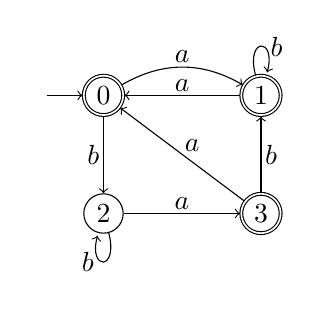
\begin{tikzpicture}[initial text={},scale=1., every node/.style={transform shape}]
		\tikzstyle{every state}=[minimum size=5mm, inner sep=0pt]
		
		\node[initial, state,accepting] (0) at (0, 0)    {$0$};
		\node[state,accepting] 		    (1) at (2,0)     {$1$};
		\node[state] 					(2) at (0,-1.5)  {$2$};
		\node[state,accepting]          (3) at (2, -1.5) {$3$};
		
		\path[->]
		(0) edge [bend left]  node [above=-0.07cm] 		 {$a$} (1)
		(0) edge 			  node [left=-0.07cm]  		 {$b$} (2)
		(1) edge 			  node [above=-0.07cm]       {$a$} (0)
		(1) edge [loop above] node [right]        		 {$b$} (1)
		(2) edge 			  node [above=-0.07cm]		 {$a$} (3)
		(2) edge [loop below] node [left]  				 {$b$} (2)
		(3) edge 			  node [above right=-0.13cm] {$a$} (0)
		(3) edge 			  node [right=-0.07cm] 		 {$b$} (1)
		;
		\end{tikzpicture}
	}\end{tabbing}\vspace{-0.5cm}\hfill$\square$
\end{example}
% how to compute next DFA

\noindent Given an enumeration state $s_{\nSO, \kAL, \nF} = (F_F, F_\delta)$ we will then compute the next DFA based on this state as described in the following algorithm. We assume, that adding $1$ to a $n$-ary number $n-1\ n-1\ \ldots n-1$ yields $00\ldots0$.
\vspace{0.2cm}
\begin{algorithmic}[1]
	\Function{IncrementEnumProgress\ }{$F_F, F_\delta, \nSO, \kAL, \nF$}
	\State add $1$ to $(F_\delta)_\nSO$
	\If {$F_\delta = 0 \ldots 0$}
		\If {$F_F = 1\ldots10\ldots0$ \textbf{and} $\#_1(F_F) = \nF$}
			\State \Return $\bot$
		\EndIf
		\While {$\#_1(F_F) \neq \nF$}
			\State add $1$ to $(F_F)_2$
		\EndWhile
	\EndIf
	\State \Return $F_F, F_\delta$
	\EndFunction
\end{algorithmic}
\vspace{0.2cm} We will treat both fields as numbers, $F_F$ as $2$-ary and $F_\delta$ as $\nSO$-ary. To get to the next DFA, we will first increment $F_\delta$ by $1$. If all transitions functions have been enumerated ($F_\delta$ becomes $0\ldots0$), then we increment $F_F$ until it contains $\nF$ $1$'s (again) and enumerate all transition functions again.

Concerning the terminating behavior of \textsc{IncrementEnumProgress} consider the following observation:

% finite enumerations, how many

\begin{observation}
	An enumeration of DFAs given $\nSO, k, \nF$ will eventually terminate. Having a requirement of $\nF$ final states, then $\binom{\nSO}{\nF}$ is the number of possible $F$-configurations. On the other hand there are $\nSO^{\nSO\kAL}$ possible $\delta$-configurations: We have to choose one of $\nSO$ possible end states for every combination in $Q\times\Sigma$ - so $\nSO\kAL$ times.
\end{observation}

\noindent This leads us to the range of an enumeration which can be expressed using the first and last enumeration state:
\begin{itemize}
	\item $s_{\nSO, \kAL, \nF} = (F_F, F_\delta) = (0\ldots0\underbrace{1\ldots 1}_{\nF\ 1's},\ 0\ldots0)$
	\item $s_{\nSO, \kAL, \nF} = (F_F, F_\delta) = (\underbrace{1\ldots 1}_{\nF\ 1's}0\ldots0,\ \nSO-1 \ldots \nSO-1)$
\end{itemize}
Consequently the algorithm can terminate in two ways. Either a next DFA could be enumerated or all DFAs with $|Q|=\nSO, |\Sigma|=k, |F|=\nF$ have been found.

%As a consequence we will create enumeration states $F_F,F_\delta$ to concrete values of $\nSO, k, \nF$ only if DFAs of that kind are requested.

%The algorithm may terminate in two ways. Either $F_F, F_\delta$ have been successfully incremented, then line 9 is reached. Or $F_F = 1\ldots 1$ and $F_\delta = \nSO-1 \ldots \nSO-1$. Then $F_\delta$ becomes $0\ldots 0$ after incrementing and $F_F$ does not reach a state with $\nF$ $1$'s again through increment --- in this case all DFAs with $|Q|=\nSO, |\Sigma|=k, |F|=\nF$ have been enumerated.

% EX -- example of an enumProgress increment
	
\begin{example}
	We showcase a sample enumeration at points, that demonstrate the semantics of different increments. We will use $\nSO=4$, $\kAL=2$ and $\nF=2$. Note that we will use $a,b,\ldots$ instead of $0,1,\ldots$ as symbols. Valid enumeration progresses are depicted green.\par
	\vspace{0.4cm}\noindent
	\begin{minipage}{0.56\textwidth}
		We will start with the initial enumeration progress (1). In this case, a simple addition of $1$ to $F_\delta$ does not cause an overflow of $F_\delta$ (2), meaning the enumeration increment is already finished.\newline
		
		(3). In this state however $F_\delta$ becomes $0\ldots0$ (4) after adding $1$. Thus we add $1$ to $F_F$, until it contains the required number of ones again (so we always have $f$ final states). The next $4$-ary number with $2$ ones after $0011$ is $0101$ (5).\newline
		
		(6). Here $F_\delta$ is at its maximum and there is no higher $4$-ary number with $2$ ones. Thus the next enumeration step yields the state (7), that marks the enumeration end.
	\end{minipage}
	\hfill
	\begin{minipage}{0.4\textwidth}
		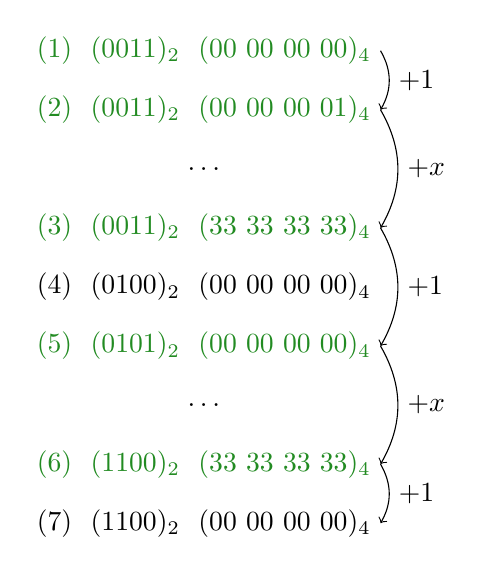
\begin{tikzpicture}
		\node (0) at (0,0) {\color{ForestGreen} (1)\ \ $(0011)_2\ \ (00\ 00\ 00\ 00)_4$} ;
		\node (1) at (0,-0.75) {\color{ForestGreen} (2)\ \ $(0011)_2\ \ (00\ 00\ 00\ 01)_4$} ;
		\node (2) at (0,-1.5) {$\ldots$} ;
		\node (3) at (0,-2.25) {\color{ForestGreen} (3)\ \ $(0011)_2\ \ (33\ 33\ 33\ 33)_4$} ;
		\node (4) at (0,-3) {(4)\ \ $(0100)_2\ \ (00\ 00\ 00\ 00)_4$} ;
		\node (5) at (0,-3.75) {\color{ForestGreen} (5)\ \ $(0101)_2\ \ (00\ 00\ 00\ 00)_4$} ;
		\node (6) at (0,-4.5) {$\ldots$} ;
		\node (7) at (0,-5.25) {\color{ForestGreen} (6)\ \ $(1100)_2\ \ (33\ 33\ 33\ 33)_4$} ;
		\node (8) at (0,-6) {(7)\ \ $(1100)_2\ \ (00\ 00\ 00\ 00)_4$};
		
		\path[->]
		(0.east) edge [bend left] node [right] {$+1$} (1.east)
		(1.east) edge [bend left] node [right] {$+x$} (3.east)
		(3.east) edge [bend left] node [right] {$+1$} (5.east)
		(5.east) edge [bend left] node [right] {$+x$} (7.east)
		(7.east) edge [bend left] node [right] {$+1$} (8.east)
		;
		\end{tikzpicture}
	\end{minipage}\par
	\hfill$\square$
\end{example}

\noindent Based on the incremented bit-fields the new DFA can be build according to the semantics defined above:
\vspace{0.2cm}
\begin{algorithmic}[1]
	\Function{DFAfromEnumProgress\ }{$F_F, F_\delta, \nSO, \kAL, \nF$}
	\State $Q \gets [[\nSO]]$
	\State $\Sigma \gets [[\kAL]]$
	\State $\delta \gets \emptyset$
	\For {$i$ \textbf{in} $[[\nSO]]$}
		\For {$j$ \textbf{in} $[[\kAL]]$}
            \State $\delta(i, j) = F_\delta[i * \kAL + j]$
		\EndFor
	\EndFor
	\State $s \gets 0$
	\For {$i$ \textbf{in} $[[\nSO]]$}
		\If {$F_F[i] = 1$}
			\State Add $i$ to $F$
		\EndIf
	\EndFor
	\State \Return $(Q, \Sigma, \delta, s, F)$
	\EndFunction
\end{algorithmic}
\vspace{0.2cm}

% saving enumProgress for later progression

\noindent Since it is not sensible to create initial enumeration states for all possible enumeration (there are infinite many, due to $\nSO\in\mathbb{N}$) we will create states by demand.

Once the enumeration to the next DFA within a call of \textsc{GenNewMinimalDFA} has been finished, it is reasonable to save the enumeration state, such that during the next call enumeration can be resumed from that point on. We will run a different enumeration for every parameter combination. Thus we introduce a second database DB$_{states}$ with the following table:
\begin{center}
	\begin{tabular}{c c c c c c c}
		$|Q_A|$ & |$\Sigma_A$| & $F_F$ & $F_\delta$ & $d_{min}$ & $d_{max}$ & $planar$
	\end{tabular}
\end{center}
In the following variant of \textsc{GenNewMinimalDFA} it can be seen how the enumeration method is integrated:
\vspace{0.2cm}
\begin{algorithmic}[1]
	\Function{GenNewMinDFA-3b\ }{$\nSO, \kAL, \nF, d, p$}
	
		\vspace{0.2cm}
	
		\State $l \gets$ all DFAs in DB$_{found}$ matching $\nSO, \kAL, \nF, d, p$
		
		\vspace{0.2cm}
		
		\If {$\exists$ enum.\ state for $\nSO, \kAL, \nF$ in DB$_{states}$}
			\State $F_F, F_\delta \gets$ load $s_{\nSO, \kAL, \nF}$ from DB$_{states}$
		\Else
			\State $F_F,F_\delta \gets 0\ldots0\underbrace{1\ldots1}_{\nF\ 1's}, 0\ldots0$
		\EndIf
		
		\vspace{-0.2cm}
		\newpage
		\While {True}
		
			\vspace{0.2cm}
		
			\If {$F_F, F_\delta$ is finished}
				\State save $F_F, F_\delta$
				\State\Return $\bot$
			\EndIf
			\State $A_{test} \gets$ next DFA based on $F_F, F_\delta$
			
			\vspace{0.2cm}
			
			\If {$A_{test}$ not minimal \textbf{or} $d \neq \mmD(A_{test})$}
				\State \textbf{continue}
			\EndIf
			
			\If {$p = 1$ \textbf{and} $A_{test}$ is not planar}
				\State \textbf{continue}
			\EndIf
			
			\If {$A_{test}$ is isomorph to any DFA in $l$}
				\State \textbf{continue}
			\EndIf
			
			\vspace{0.2cm}
			
			\State save $F_F, F_\delta$ in DB$_{states}$
			\State save $A_{test}$ and its respective properties in DB$_{found}$
			\State\Return $A_{test}$
		\EndWhile
	\EndFunction
\end{algorithmic}
\vspace{0.2cm}

\section{Related Work on DFA Generation}

Nicaud provides an overview of results on random generation and combinatorial properties of DFAs in ~\cite{Nic14}. We will outline relevant related work.

Nicaud's summary indicates, that research has focused on randomized generation of accessible, but not minimal DFAs so far. In the following we will sketch some approaches that have come up.

\paragraph*{Using the Recursive Method.}

Champarnaud and Paranthoën~\cite{CP05} continue ideas started by Nicaud in his thesis~\cite{Nic00}. Let $\mathfrak{F_{n,m}}$ be the set of extended $m$-ary trees of order $n$. These trees are characterized by a partitioning $V = N \uplus L$ with $|N| = n$ and the properties $v \in N \Rightarrow d^+(v) = m$ and $v \in L \Rightarrow d^+(v) = 0$. We define the following set of tuples using $s=n(m-1)$:
\[
    \mathfrak{R_{m,n}} = \{\ (k_1,\ldots,k_s) \in \mathbb{N}^s\ |\ \forall i\in [2,s]\colon k_i \geq \left\lceil\frac{i}{m-1}\right\rceil\ and\ k_i \geq k_{i-1}\ \}
\]
In~\cite[p. 6]{CP05} it is shown that there exists a bijection $\varphi$ between $\mathfrak{F_{n,m}}$ and $\mathfrak{R_{m,n}}$ which maps to $k_i$, $i\in[1,s]$ of a tuple the number of leaves visited before the $i$th leaf in a tree. The connection to accessible DFAs is established by proving that  ``transition structures\footnotemark''\ with $|Q|=n$, $|\Sigma|=m$ reduced to the set of the smallest paths from the $s$ to each other state are in bijection with extended $m$-ary trees of order $n$ (see~\cite[p. 8]{CP05}).

As a consequence Champarnaud and Paranthoën are able to construct a random generator of accessible complete DFAs using the ``recursive method'' from~\cite{NW78} which generates $n$-tuples~\cite[p. 10]{CP05}. Nicaud states in his survey that the algorithm's runtime is $\mathcal{O}(n^2)$ but notes, that generation of DFAs with more than ``a few thousand states'' is practically hard to do~\cite[pp. 10-11]{Nic14}.
\footnotetext{Those are essentially DFAs without final state sets.}

Almeida et al.~\cite{AAA09, AMR09, RMA05} present and implement methods using a string-encoding of DFAs for exact enumeration and random generation of DFAs. Nicaud~\cite[p. 11]{Nic14} states in a remark, that this approach uses the same recursive method and differs only in the DFA encoding.

\paragraph*{Using Boltzmann Sampler.}

Bassino, David and Nicaud present and implement a more efficient random generator of accessible complete DFAs in~\cite{BDN07, BN07}. Their idea is based on so called Boltzmann samplers. This framework of samplers is characterized in particular by the fact that the size of its generated objects are not fixed but in an interval around a given input size - this stands in opposition to most random generators in literature~\cite[p. 2]{DFL04}.

In~\cite{BN07} the authors use a Boltzmann sampler to generate set partitions that are shown to be in bijection with so called box diagrams~\cite[p. 8]{BN07} which are in turn in bijection to accessible complete DFAs~\cite[p. 4]{BN07}. They thus acquire an average runtime complexity of $\mathcal{O}(n^{1.5})$ for a single random generation.

\paragraph*{Using a Rejection Algorithm.}

Carayol and Nicaud~\cite{CN12} give a simple algorithm with the same runtime complexity ($\mathcal{O}(n^{1.5})$). They use a result stating that the size of accessible DFAs is concentrated around some computable value. In the end random (possibly inaccessible) DFAs of a specific size are generated, of which afterwards all unreachable states are deleted. This is thus essentially a rejection algorithm with clever generation of test DFAs. They furthermore show that allowing approximate sampling with the number of states being in $[n-\varepsilon\sqrt{n}, n+\varepsilon\sqrt{n}]$ results in linear expected runtime.

\paragraph*{Others and Comparison to Algorithm Presented in this Work.}

In his survey Nicaud mentions a paper by Bassino and Sportiello~\cite{BS13} that yields random generation of accessible DFAs in expected linear time. This work will not be discussed further here.

In this work we use a rejection algorithm that generates test DFAs either by randomization or by enumeration. Both methods implement a naive approach. The generated test DFAs are not necessary minimal and in particular not necessary accessible as in~\cite{CN12}. The enumeration method uses encodings of DFAs similar to those used by Almeida et.\ al.~\cite{RMA05}.


\section{Empirical and Combinatorial Results}

Concerning combinatorial properties of DFAs, several authors (e.g.~\cite{BN07, DKS02, HJ14}) consider a work from Vyssotsky~\cite{Vys59} in the Bell laboratories to be the first on this subject. A contribution by Korshunov~\cite{Kor78} is often cited in this regard, for he firstly ``determines an asymptotic estimate of the number of accessible complete and deterministic $n$-state automata over a finite alphabet''~\cite{BDS11}.

More recent implementations (e.g.~\cite{AAA09, BDN07}) of various random and enumeration generation methods have given rise to several empirical observations concerning the number of minimal DFAs, their fraction among all DFAs and so forth.

Domaratzki, Kisman, and Shallit~\cite{DKS02} give some asymptotic estimates and explicit computations for the number of several types of distinct languages and automata. The here relevant results have been subsumed and extended in~\cite[p. 8]{AMR09} and were empirically confirmed in~\cite{BDN07}.

In Figure~\ref{fig:dfa_minimal_ratios} we use these results to determine the ratios of minimal complete DFAs among all complete DFAs for given $|Q|$ and $|\Sigma|$. The number of all DFAs is computed as follows:
\[
|\mathcal{A}_{n,k}| = \underbrace{n^{n*k}}_{\#\text{possible }\delta\text{'s}} * \underbrace{2^n}_{\#\text{possible sets }F}
\]
Thus we gain an insight into how probable the random generation of a distinct minimal test DFA is without applying further constraints. For our proposed default parameters $n\in[4-5]$ and $k\in[2-3]$ the probabilities of successful generation range from $1\%$ to $5\%$. Practical tests have shown that this leads to sufficient short run times for our implementation.

Further interesting results in this area include the determination of the fraction of all minimal automata among all accessible complete DFAs~\cite{BDS11} and asymptotic estimates for the number of states that a random minimized DFA has~\cite{BK13}.

\begin{figure}[t]
	\centering
	\begin{tabular}{|c|c|l|l|l|}
		\hline
		$|\Sigma|$ ($k$) & $|Q|$ ($n$) & $|\mathcal{A}_{min,n,k}|$ & $|\mathcal{A}_{n,k}|$ & Minimal \% \\\hline
		
		$k = 2$ & $2$ & \textbf{24} & 64 & 0.38 \\
		& $3$ & \textbf{1028} & 5832 & 0.18 \\
		& $4$ & \textbf{56014} & 1048576 & 0.05 \\
		& $5$ & \textbf{3705306} & 312500000 & 0.01 \\
		& $6$ & \textbf{286717796} & 139314069504 & 0.0 \\
		& $7$ & \textbf{25493886852} & 86812553324672 & 0.0 \\\hline
		
		$k = 3$ & $2$ & \textbf{112} & 256 & 0.44 \\
		& $3$ & \textbf{41928} & 157464 & 0.27 \\
		& $4$ & \textbf{26617614} & 268435456 & 0.1 \\
		& $5$ & \textbf{25184560134} & 976562500000 & 0.03 \\\hline
		
		$k = 4$ & $2$ & \textbf{480} & 1024 & 0.47 \\
		& $3$ & \textbf{1352732} & 4251528 & 0.32 \\
		& $4$ & \textbf{7756763336} & 68719476736 & 0.11 \\\hline
		
		$k = 5$ & $2$ & \textbf{1984} & 4096 & 0.48 \\
		& $3$ & \textbf{36818904} & 114791256 & 0.32\\\hline
	\end{tabular}
	\caption{Table depicting the exact amount of minimal complete DFAs among all complete DFAs for various sizes of $Q, \Sigma$. The numbers of minimal DFAs (bold numbers) are taken from~\cite[p. 8]{AMR09}.}
	\label{fig:dfa_minimal_ratios}
\end{figure}

	% !TeX spellcheck = en_US

\chapter{Extending minimal DFAs} \label{ch:4}

We firstly define a formal problem for extending a minimal DFA $A_{sol}$ to a task DFA $A_{task}$ based on our requirements analysis (see~\ref{ch:1:requirements-analysis}):
\begin{definition}[ExtendMinimalDFA] $ $ \\
	$ $ \vspace{-0.cm} \\
	\noindent $\underline{\emph{Given:}}$
	\vspace{-0.2cm}
	\begin{align*}
	A_{sol} = (Q, \Sigma, \delta, s, F) \in \Amin\ \ \ & \emph{solution DFA} \\
	\nEQ \in \mathbb{N}\ \ \ & \emph{number of states creating equivalent state pairs} \\
	\nUN \in \mathbb{N}\ \ \ & \emph{number of unreachable states} \\
	p \in \{0,1\}\ \ \ & \emph{planarity-bit} \\
	c \in \{0,1\}\ \ \ & \emph{completeness-bit}
	\end{align*}
	\noindent $\underline{\emph{Task:}}$ \emph{Compute, if it exists, a task DFA $A_{task}$ with}
	\begin{itemize}
		\item $Q_{task} = Q_{sol} \cup \{ r_1, \ldots, r_\nEQ, u_1, \ldots, u_\nUN \}$
		\item $r_1, \ldots, r_\nEQ$ \emph{each creating an equivalent state pair}
		\item $u_1, \ldots, u_\nUN$ \emph{unreachable}
		\item $\Sigma_{task} = \Sigma_{sol}$, $s_{task} = s_{sol}$, $F_{task} \subseteq F_{sol}$
		\item $A_{task}$ \emph{being planar iff} $p = 1$
		\item $A_{task}$ \emph{being complete iff} $c = 1$
		\item $A_{sol}$ \emph{being isomorph to} $\MinAlg(A_{task})$
	\end{itemize}
\end{definition}
\noindent In order to fulfill these requirements we will deduce for both kinds of states how they may be added by examining their desired properties. We will show for the action of adding equivalent states, that this does not change a DFAs $\mmD$-value.

\section{Creating equivalent state pairs}

Step 3 and 4 of the minimization algorithm are concerned with detection and elimination of equivalent state pairs. We now want to add states $r_1,\ldots,r_\nEQ$ to a DFA $A_{sol}$, gaining $A_{re}$ with $Q_{re} = Q_{sol} \cup \{r_1,\ldots,r_\nEQ\}$, such that each of these states is equivalent to a state in $A_{re}$. Note that, for reasons of clarity, we are going to abbreviate from now on $A_{re} = A$, $Q_{re} = Q$, $\sim_{A_{re}} = \sim_A$ etc.

%At this point we notice, that $A_{sol}$ is isomorph to the $\sim$-equivalence automaton (see def.~\ref{ch:1:sim-eq-dfa}). We can think 

Consider the properties $r_1,\ldots,r_\nEQ$ must have. They are equivalent to states $o_1,\ldots,o_\nEQ$ of $A$.
\[
\exists r_1,\ldots,r_\nEQ \in Q\colon\ \exists o_1,\ldots,o_\nEQ \in Q\colon\ \forall i \in [1,\nEQ] \colon\ r_i \sim_A o_i
\]
But we know also and in particular, that each of them is equivalent a state $e$ of $A_{sol}$.
\[
	\exists r_1,\ldots,r_\nEQ \in Q\colon\ \forall i \in [1,\nEQ] \colon\ \exists e \in Q_{sol}\colon\ r_i \sim_A e
\]
In our algorithm, we will choose the state $e$ for each state we add.

\subsection{Adding outgoing transitions}

Regarding the outgoing transitions of any $r_i$ equivalent to a state $e$, we are directly restricted by the relationship $\forall \sigma \in \Sigma \colon [\delta(r_i, \sigma)]_{\sim_A} = [\delta(e, \sigma)]_{\sim_A}$. Thus, when adding some $r_i$, we have to choose for each symbol $\sigma \in \Sigma$ at exactly one transition (completeness requirement for $A$) from the following set:
\[
	O_{e,\sigma} = \{\ ((r_i, \sigma), q)\ |\ q \in [\delta(e, \sigma)]_{\sim_A}\ \}
\]
Since the solution DFA is complete and since every here added state gets a transition for every alphabet symbol, we know that every $O_{e,\sigma} \neq \emptyset$.

\gregor{Why does this not affect the eq. class of any other state?}

\subsection{Adding ingoing transitions}

First of all, we know, that $r_i$ is reachable, since every state of $A$ must be reachable, so we need to give $r_i$ at least one ingoing transition. Doing this, we have to ensure, that any state $q$, that gets such an outgoing transition to $r_i$ remains in its $\sim$-equivalence class.
	
Thus a fitting state $q$ has to have a transition to some state in $[r_i]_{\sim_A} = [e]_{\sim_A}$ already. So, given a state $q$ with $\delta(q, \sigma) = p$ and $p \in [e]_{\sim_A}$, we can set $\delta(q, \sigma) = r_i$ and thus ``steal'' $q$ its ingoing transition.

We see here, that $q$ must have at least $2$ ingoing transitions, else it would become unreachable. Thus we summarize:
\[
    I_e = \{\ ((q, \sigma), p)\ |\ \delta(q, \sigma) = p \land p \in [e] \land d^-(p) \geq 2\ \}
\]
Choose at least one $((q, \sigma), p) \in I_e$, remove $((q, \sigma), p)$ from $\delta$ and add $((q, \sigma), r_i)$. 

These finding lead us to a general requirement regarding the choice of a state $e$ for an $r_i$: The equivalence class of any $e$ has to contain at least one state with at least $2$ ingoing transitions (see fig.~\ref{fig:dfa_create_equivalent_states}). We establish the following notion to pin down this restriction:
\[
	duplicatable(q) \Leftrightarrow_{def} (\exists p \in [q]_{\sim_A}\colon |d^-(p)| \geq 2)
\]
The number of duplicatable states in any accessible DFA $A$ is $0$ for $|\Sigma| \leq 1$ (due to the restriction $|d^-(p)| \geq 2$) and greater than $0$ for $|\Sigma| > 1$ due to the pigeonhole principle: An accessible complete DFA has $|Q||\Sigma|$ transitions which have to be spread across $|Q|$ states.
\begin{example}
	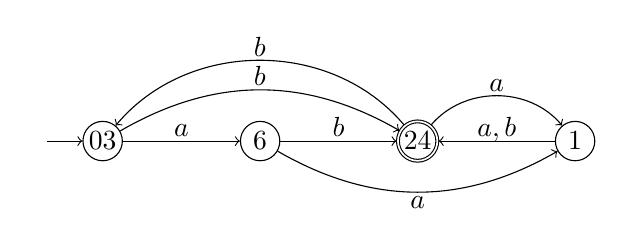
\begin{tikzpicture}[initial text={},scale=1., every node/.style={transform shape}]
	\tikzstyle{every state}=[minimum size=5mm, inner sep=0pt]
	
	\node[initial, state]  (03) at (0, 0)   {$03$};
	\node[state] 		   (1) at (6, 0)   {$1$};
	\node[state,accepting] (24) at (4,0)    {$24$};
	\node[state]           (6) at (2,0)    {$6$};
	
	\path[->]
	(03) edge node [above=-0.07cm]  {$a$}   (6)
	(03) edge [bend left] node [above=-0.07cm]  {$b$}   (24)
	
	(1) edge node [above=-0.13cm]  {$a,b$}   (24)
	
	(24) edge [bend left=50] node [above=-0.07cm]  {$a$}   (1)
	(24) edge [bend right=50] node [above=-0.07cm]  {$b$}   (03)
	
	(6) edge [bend right] node [below=-0.07cm]  {$a$}   (1)
	(6) edge node [above=-0.07cm]  {$b$}   (24)
	;
	\end{tikzpicture}
\end{example}
\begin{figure}
	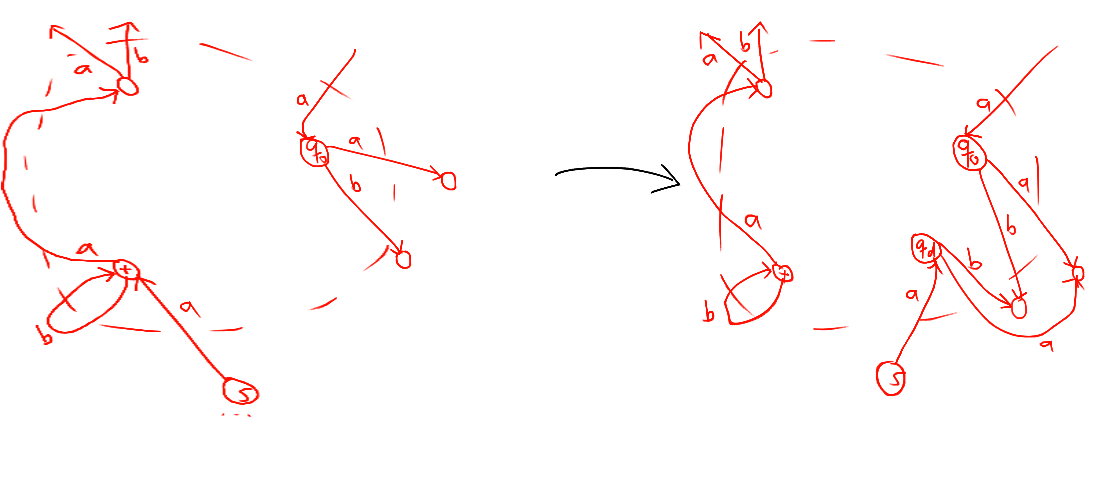
\includegraphics[width=\linewidth]{images/dfa_create_equivalent_states.png}
	\caption{If an equivalence class (here denoted by the states in the dashed area) contains a state with 2 or more ingoing transitions (in this case $p$), then a state equivalent to any of the classes states may be added. Here $r$ is equivalent to $o$ and is ``stealing'' the ingoing transition $\delta(q, a)$ from $p$.}
	\label{fig:dfa_create_equivalent_states}
\end{figure}

\subsection{The algorithm}

\vspace{0.2cm}
\begin{spacing}{1}
\begin{algorithmic}[1]
	\Function{CreateEquivalentStatePairs}{$A, \nEQ$}
    \State $Q \gets Q_{sol}$
    \State $\delta \gets \delta_{sol}$
    \State $F \gets F_{sol}$
	\State $K \gets \{\ \{q\}\ |\ q \in Q\ \}$ \Comment{tracks the equivalence classes of $A$}
	\State $k(q) = C$ such that $q \in C$ and $C \in K$ \Comment{returns the equivalence class to $q$}
	\State $in(q) = |d^-(q)|$ for all $q \in Q$ \Comment{tracks the number of ingoing t.}
	
    \For {$i$ \textbf{in} $[1,\nEQ]$}
		\For {$q$ \textbf{in} $Q$} \Comment{find a duplicatable state $e$}
			\If {$in(q) \geq 2$}
				\State $e \gets$ random chosen state from $k(q)$
				\State \textbf{break}
			\EndIf
		\EndFor
		
		\State $r_i \gets$ unused state label \Comment{create to $e$ equivalent state $r_i$}
        \State Add $r_i$ to $Q$
		\State Add $r_i$ to $k(e)$
		
		\For {$\sigma$ \textbf{in} $\Sigma$} \Comment{add $d^+(r_i)$}
			\State $\delta(r_i, \sigma) =$ random chosen state from $k(\delta(e, \sigma))$
		\EndFor
		
		\State $P \gets \{\ ((s, \sigma), t) \in \delta\ |\ t \in k(e),\ in(t) \geq 2\ \}$ \Comment{add $d^-(r_i)$}
		\State $C \gets$ random nonempty subset of $P$
		\For {$((s, \sigma), t)$ \textbf{in} $C$}
			\State $in(t) \gets in(t) - 1$
			\State $in(r_i) \gets 1$
            \State $\delta(s, \sigma) = r_i$
		\EndFor
	\EndFor
    \State \Return $(Q, \Sigma_{sol}, \delta, s_{sol}, F)$
	\EndFunction
\end{algorithmic}
\end{spacing}
\vspace{0.2cm}
\noindent Note that computing an unused state label can be easily done by e.g.\ taking the maximum of all solution DFA states (which are nothing else but numbers) and adding one.

\subsection{The existence of equivalent state pairs does not affect D} \label{ch:3:sec-D-proof}

To prove this statement, we will first introduce two auxiliary definitions and prove two minor propositions.

A word $w$ shall be called \emph{finishing word of $q$}, iff $\delta^*(q, w) \in F$. With $f(q) = \{\ w\ |\ \delta^*(q, w) \in F\ \}$ we denote the set of all finishing words to a state.
\begin{definition} \label{ch:4:def-dist-word}
	We will call a word $w$ \emph{distinguishing word of $p,q$}, iff $d_A(w, p, q)$ is true where
	\begin{align*}
	d_A(w, p, q) \text{ is true} &\Leftrightarrow (\delta^*(p,w) \in F \Leftrightarrow \delta^*(q,w) \notin F) \\
	&\Leftrightarrow (w \in f(p) \Leftrightarrow w \notin f(q))
	\end{align*}
\end{definition}
\noindent The following lemma and its proof are in parts inspired by Martens and Schwentick \cite[ch.\ 4 p.\ 18]{MS18}.

\begin{lemma}\label{ch:3:semantics-of-m(n)}
    In the context of \CompDist\ the following is true: If and only if $(p,q)\in m(n)$, the shortest distinguishing word of $p,q$ has length $n$. Formally:
    \begin{align*}
        (p,q) \in m(n) \Longleftrightarrow\ &\exists w\in\Sigma^*\colon (|w| = n\ \land d_A(w, p, q))\\
        \land\ &\nexists v\in\Sigma^*\colon (|v| < n\ \land d_A(v, p, q))
    \end{align*}
\end{lemma}

\begin{proof}
	Per induction on the number of \CompDist-iterations $n$.
	
	\paragraph*{$n = 0$, ``$\Leftrightarrow$''.}
	\begin{align*}
		&(p,q) \in m(0) = \{ (p,q), (q,p)\ |\ p \in F, q \notin F \}\hfill\text{ (see alg.~\ref{ch:1:m-minmark}, line 2))}\\
		\Leftrightarrow\ &\text{one of $p,q$ in $F$, one not}\\
		\Leftrightarrow\ &\text{one of $\delta^*(p, \varepsilon),\delta^*(q, \varepsilon)$ in $F$, one not}\\
		\Leftrightarrow\ &\exists w\in\Sigma^*\colon (|w|=0\land\text{one of $\delta^*(p, w),\delta^*(q, w)$ in $F$, one not})\\
		\Leftrightarrow\ &\exists w\in\Sigma^*\colon (|w| = 0\ \land d_A(w, p, q))\\
		&\text{and there is no shorter such word }\checkmark
	\end{align*}
	
	\paragraph*{$0\ldots n-1 \rightarrow n$, ``$\Rightarrow$''.} 
	Then the following holds for some states $p,q$ (see alg.~\ref{ch:1:m-minmark}, line 5):
	\begin{equation}\label{ch:3:eq:m(n)}
		(p,q) \in m(n) = \{ (p,q), (q,p)\ |\ (p,q) \notin \bigcup{m(\cdot)} \land \exists \sigma \in \Sigma \colon (\delta(p,\sigma), \delta(q,\sigma)) \in m(n-1) \}
	\end{equation}
	So, in particular there exists a symbol $\sigma$ such that $(\delta(p,\sigma),\delta(q,\sigma)) \in m(n-1)$. Let $(p',q')=(\delta(p,\sigma),\delta(q,\sigma))$, so $(p',q')\in m(n-1)$.
	
	Per induction there exists a shortest distinguishing word $w'$, $|w'|=n-1$ to $p',q'$. Thus one of $\delta^*(p', w'),\delta^*(q', w')$ is in $F$, one not and there is no shorter word.
	
	Thus one of $\delta^*(p, \sigma w'),\delta^*(q, \sigma w')$ is in $F$, one not, which makes $\sigma w'$ a distinguishing word of length $n$ for $p,q$.
	
	Since $(p,q)$ is not in any $m(i), i<n$ (recall $(p,q) \notin \bigcup{m(\cdot)}$ of eq.~\ref{ch:3:eq:m(n)}), there is per induction no shorter distinguishing word.\ $\checkmark$ 
	
	\paragraph*{$0\ldots n-1 \rightarrow n$, ``$\Leftarrow$''.} 
	Then the following holds for some states $p,q$:
	\begin{align*}
	&\exists w\in\Sigma^*\colon (|w| = n\ \land d_A(w, p, q))\\
	\land\ &\nexists v\in\Sigma^*\colon (|v| < |w|\ \land d_A(v, p, q))
	\end{align*}
	So there exists a word $w$ with $|w|=n>0$ such that one of $\delta^*(p, w),\delta^*(q, w)$ is in $F$, one not and there is no shorter word fulfilling this property.
	
	Since $w$ is non-empty there exists a symbol $\sigma$ such that $w = \sigma w'$. Let $(\delta(p,\sigma),\delta(q,\sigma)) = (p',q')$.
	
	Thus, if one of $\delta^*(p, \sigma w'),\delta^*(q, \sigma w')$ is in $F$ and one not, then the same must hold for $\delta^*(p', w'),\delta^*(q', w')$, so $w'$ is a distinguishing word for $p',q'$.
	
	It is also the shortest one, because, if there existed a shorter word $v'$, $|v'| < |w'|$, then $\sigma v'$ would be a distinguishing word shorter than $w$ for $p,q$ which is contradictory.
	
	Since $w'$ is a shortest distinguishing word for $p',q'$, we may deduce now per induction, that $(p',q')\in m(n-1)$.
	
	The pair $(p,q)$ is not in any $m(i)$, $i<n$, since otherwise per induction the shortest distinguishing word would be shorter than $w$ and thus not $w$. Since $(p',q')\in m(n-1)$ and $(\delta(p,\sigma),\delta(q,\sigma)) = (p',q')$, we can then deduce by the definition of $m$, that $(p,q)\in m(n)$.\ $\checkmark$ 
\end{proof}

\begin{lemma}\label{ch:3:semantics-of-D(A)}
    If \CompDist\ has done $\mmD(A)$ iterations and terminated, then the longest word $w$, that is a shortest distinguishing word for any state pair, has length $\mmD(A)-1$.
\end{lemma}

\begin{proof}
	Via direct proof. Assume $m$-\CompDist(A) has done $n$ iterations (so $\mmD(A) = n$). We observe, that
	\begin{enumerate}
		\item $\forall i \in [0,n-1]\colon m(i) \neq \emptyset$
		\item $m(n)= \emptyset$
		\item $\forall i > n\colon m(i)= \bot$\ .
	\end{enumerate}
	This follows directly from while loop and its terminating condition of \CompDist (alg.~\ref{ch:1:m-minmark}, line 4--7). Given this, we will prove: There exists a shortest distinguishing word of length $n-1$ for some state pair, but a longer such word can not exist.
    
%    Recall Lemma~\ref{ch:3:semantics-of-m(n)}:
%    \begin{align*}
%    (p,q) \in m(n) \Longleftrightarrow\ &\exists w\in\Sigma^*\colon (|w| = n\ \land d_A(w, p, q))\\
%    \land\ &\nexists v\in\Sigma^*\colon (|v| < |w|\ \land d_A(v, p, q))
%    \end{align*}

	% a possible word per definition of D(A), m(i) and lemma
	
	Following Lemma~\ref{ch:3:semantics-of-m(n)} and the first observation, we can deduce the existence of a shortest distinguishing word $w$ with $|w| = n-1 = \mmD(A)-1$ for some $p,q \in Q$.
	
	% There is no word longer than that
	
	There cannot be any shortest distinguishing word $w'$ with $|w'| = k > n-1$ for any two states $p',q'\in Q$. Following Lemma~\ref{ch:3:semantics-of-m(n)} again, $m(k)$ for some $k > n-1$ would be defined and non-empty, which is contradictory to observations 2 and 3.
\end{proof}

%\begin{lemma}\label{ch:3:lem:disting-trans}
%	If $w$ is shortest distinguishing word for $p,q$ and $q \sim_A q'$, then $w$ is a shortest distinguishing word for $p,q'$.
%%    \[
%%    d_A(w, p, q) \land q \sim_A q' \Rightarrow d_A(w, p, q')
%%    \]
%\end{lemma}
%
%\begin{proof}
%    Via direct proof. The relation $q \sim_A q'$ says that for all words $z$, $\delta^*(q,z)$ and $\delta^*(q',z)$ are both in $F$ or both not in $F$. Consequently asking whether the following is true
%    \[
%    	\delta^*(p,z)\in F \Leftrightarrow \delta^*(q,z)\in F
%    \]
%    is the same as asking whether this is true:
%    \[
%    	\delta^*(p,z)\in F \Leftrightarrow \delta^*(q',z)\in F
%    \]
%    This implies, that $q$ and $q'$ have exactly the same distinguishing words with other states (see definition of distinguishing words). As a consequence they too have the same shortest distinguishing words with other states.
%\end{proof}

\begin{theorem}
	Given two accessible DFAs $A$, $A'$. If their language is the same ($L(A) = L(A')$), then $\mmD(A) = \mmD(A')$.
\end{theorem}

\begin{proof}
	Per direct proof. Starting with the language-equivalence of $A$ and $A'$ we observe, that the start states of both DFAs have the same finishing words.
	\vspace{0.25cm}
	\begin{itemize}
		\item[] $L(A) = L(A')$
		
		\item[$\Rightarrow$] $\{\ w\ |\ \delta^*(s, w) \in F\ \} = \{\ w\ |\ \delta'^*(s', w) \in F'\ \}$
		
		\item[$\Rightarrow$] $\forall w \in \Sigma^*\colon \delta^*(s, w) \in F \Leftrightarrow \delta'^*(s', w) \in F'$
	\end{itemize}
	We extend this to a statement that includes any state visited on the way to $F$ resp.\ $F'$.
	\begin{itemize}
		\item[] $\forall u \in \Sigma^*\colon \forall v \in \Sigma^*\colon$
		
		\qquad $\delta^*(s, u) = q \land \delta'^*(s', u) = q' \land$
		
		\qquad $(\delta^*(q, v) \in F \Leftrightarrow \delta'^*(q', v) \in F')$
	\end{itemize}
	Through shifting the second quantor directly before the last line we can now see, that those states reached by the same word in $A$, $A'$ have the same finishing words.
	\begin{itemize}
		\item[] $\forall u \in \Sigma^*\colon \forall v \in \Sigma^*\colon$
		
		\qquad $\delta^*(s, u) = q \land \delta'^*(s', u) = q' \land$
		
		\qquad $(\forall v \in \Sigma^*\colon (\delta^*(q, v) \in F \Leftrightarrow \delta'^*(q', v) \in F'))$
		
		\item[$\Rightarrow$] $\forall u \in \Sigma^*\colon$
		
		\qquad $\delta^*(s, u) = q \land \delta'^*(s', u) = q' \land$
		
		\qquad $f(q) = f(q')$
	\end{itemize}
	Since we are making a statement about all states reached from $s$/$s'$ and since all states in $A$/$A'$ are reachable, we may conclude:
	
	For every state in $A$/$A'$ there exists a state in the other DFA, such that their finishing words are equal.
	\begin{itemize}
		\item [] $\forall q \in Q\colon \exists q' \in Q'\colon f(q) = f(q')$ \hfill $\land$ \hfill $\forall q' \in Q'\colon \exists q \in Q\colon f(q') = f(q)$ \qquad \qquad \qquad \qquad
		
		\item[$\Rightarrow$] $\{\ f(q)\ |\ q \in Q\ \} = \{\ f(q')\ |\ q' \in Q'\ \}$
	\end{itemize}
	Since every distinguishing word is a finishing word (see def.~\ref{ch:4:def-dist-word}), there cannot be a distinguishing word in one of $A$/$A'$, that is not distinguishing word in the other DFA.
	
	As a consequence both DFAs have the same shortest distinguishing words and thus too the same longest shortest distinguishing word.
	
	If $\mmD(A) \neq \mmD(A')$ then by Lemma~\ref{ch:3:semantics-of-D(A)} one DFA would have a longer longest shortest distinguishing word, which is not possible as proven, thus $\mmD(A) = \mmD(A')$ must be true. 
\end{proof}

\section{Adding unreachable states}

From step 1 of the minimization algorithm we can deduce how to add unreachable states. These can easily be added to a DFA by adding non-start states with no ingoing transitions (see def.~\ref{ch:1:unreachable-states}). Number and nature of outgoing transitions may be arbitrary.

\vspace{0.2cm}
\begin{algorithmic}[1]
	\Function{AddUnreachableStates\ }{$A, \nUN, c$}
	\For {$\nUN$ \textbf{times}}
		\State $q \gets$ unused state label
		\State $Q \gets Q \cup \{ q \}$
        \State $outSymbols \gets c = 1\ ?\ \Sigma\ :\ $ random subset of $\Sigma$
		\State $R \gets$ random chosen sample of $|outSymbols|$ states from $Q \setminus \{q\}$
		\For {$\sigma$ \textbf{in} $outSymbols$}
			\State $q' \in R$
			\State $R \gets R \setminus \{q'\}$
			\State $\delta \gets \delta \cup \{ ((q, \sigma), q') \}$
		\EndFor
	\EndFor
	\State \Return $A$
	\EndFunction
\end{algorithmic}
\vspace{0.2cm}
If completeness is demanded ($c=1$), then we set $\Sigma$ as set of all symbols, for which a state shall gain outgoing transitions. Else we choose a random subset for each state, such that some unreachable states may miss some outgoing transitions.

	\chapter{Conclusion}

What happens, if we change start and accepting states? \\
What happens, if we add transitions only? \\

\noindent dfa specific planarity test? \\
use planarity test information for better drawing?
	
	\appendix
	% List of figures, theorems/lemmas/etc., bibliography, index
	
	\nocite{*}
	\bibliographystyle{abbrv}
	\bibliography{thesis}
	
	\chapter*{Erklärung}
	\addcontentsline{toc}{chapter}{Erklärung}
	
	Hiermit versichere ich, Gregor Hans Christian Sönnichsen, dass ich die vorliegende Arbeit selbständig verfasst habe, keine anderen als die von mir angegebenen Quellen und Hilfsmittel benutzt habe und die Arbeit nicht  bereits zur Erlangung eines akademischen Grades eingereicht habe. \\
	
	\noindent Bayreuth, den 8.\ Februar 2020. \\\\\\\\\\\\\\
	\noindent Gregor Hans Christian Sönnichsen

\end{document}          
